\documentclass[12pt]{article}

% ---------------------------------------------------------------------------
% Estimation and Inference on Two-Threshold Value Functionals -- VERSION 2
% ---------------------------------------------------------------------------
% Standalone-compilable companion to may_2026.tex ("Inference on Policy Value
% under Admissibility-Constrained Optimal Treatment Rules").  Designed to slot
% in as the "Estimation and Inference of the Value Functional" section of the
% JMP: it generalizes Chen, Chen & Gao (2025) [single threshold: plug-in,
% analytical variance, sieve-Riesz inference] and the extended draft
% [quadratic debiasing, sieve DML] to value functionals defined by TWO
% thresholds, and develops the combined (doubly debiased) procedure left open
% in Remark 7 of the extended draft.  Macros match may_2026.tex.
%
% v2 changes (see "Revision note" after the abstract):
%   * corrected order accounting for the second-order diagonals
%   * corrected corner-bias coefficient (adds the cos(omega) diagonal pieces)
%   * corrected/strengthened statements of Lemma jackknife, Prop margins,
%     Thm ss, Thm dml, Thm dd; explicit assumption lists
%   * corrected Riesz band display (missing v_0 f / f_0 weight)
%   * explicit empirical-measure variance term
%   * new Appendix C (numerical verification of Theorem D2)
%   * new Section 6.5 on what the current Monte Carlo does and does not show
%   * real bibliography
% ---------------------------------------------------------------------------

\usepackage[margin=1in]{geometry}
\usepackage{setspace}
\usepackage{amsmath,amssymb,amsthm,mathtools,bm}
\usepackage{enumitem}
\usepackage{natbib}
\usepackage[colorlinks=true,linkcolor=blue,citecolor=blue,urlcolor=blue]{hyperref}
\usepackage{booktabs}
\usepackage{longtable}
\usepackage{graphicx}
\usepackage{microtype}
\usepackage{bbm}
\usepackage{array}

\onehalfspacing

\newtheorem{theorem}{Theorem}[section]
\newtheorem{proposition}[theorem]{Proposition}
\newtheorem{lemma}[theorem]{Lemma}
\newtheorem{corollary}[theorem]{Corollary}
\newtheorem{assumption}[theorem]{Assumption}
\newtheorem{definition}[theorem]{Definition}
\newtheorem{remark}[theorem]{Remark}
\newtheorem{example}[theorem]{Example}

\newcommand{\R}{\mathbb{R}}
\newcommand{\E}{\mathbb{E}}
\newcommand{\Prob}{\mathbb{P}}
\newcommand{\1}{\mathbbm{1}}
\newcommand{\dd}{\,\mathrm{d}}
\newcommand{\Haus}{\mathcal{H}}
\newcommand{\norm}[1]{\left\lVert #1 \right\rVert}
\newcommand{\abs}[1]{\left\lvert #1 \right\rvert}
\newcommand{\inner}[2]{\left\langle #1, #2 \right\rangle}
\newcommand{\argmax}{\operatorname*{arg\,max}}
\newcommand{\Th}{\Theta}
\newcommand{\Mg}{\mathcal{M}_{g}}
\newcommand{\Mh}{\mathcal{M}_{h}}
\newcommand{\Corner}{\mathcal{C}}
\newcommand{\Ng}{\norm{\nabla g_{0}}}
\newcommand{\Nh}{\norm{\nabla h_{0}}}

\title{Estimation and Inference on Two-Threshold Value Functionals\thanks{%
This section extends the single-threshold framework of \citet{ccg2025} and its
debiased-estimation companion to value functionals defined by the intersection
of two estimated decision boundaries. It is written to be self-contained;
notation follows the JMP draft \texttt{may\_2026.tex}.}}
\author{Zhenxiao Chen\thanks{Department of Economics, University of
Pennsylvania, USA, zxchen@upenn.edu.}}
\date{\today\\[4pt]\normalsize Version 2}

\begin{document}
\maketitle

\begin{abstract}
\noindent We study estimation and inference for value functionals of the form
$\Th_{0}=\E\big[\1\{g_{0}(X)\geq0\}\,\1\{h_{0}(X)\geq0\}\,v_{0}(X)\big]$,
where $g_{0}$ and $h_{0}$ are two nonparametric contrast functions estimated
from the same experiment. Such \emph{two-threshold} functionals arise whenever
a planner imposes a pointwise admissibility screen on top of a benefit margin:
leading examples are the share of the population that benefits in the short
run but is harmed in the long run under a surrogate-index treatment rule
\citep{acik2024}, and treatment-path welfare components
of an optimal dynamic regime. We generalize the single-threshold theory of
\citet{ccg2025}: the pathwise derivative is a sum of \emph{two}
boundary (Hausdorff) integrals, the plug-in estimator converges at the
one-dimensional nonparametric rate $n^{-s/(2s+1)}$ (attained under
$s\geq d$), and a two-band sieve-Riesz
variance estimator delivers valid studentized inference. Our main new result
characterizes the \emph{second-order} pathwise derivative: in addition to two
margin curvature terms it contains a codimension-two \emph{corner} integral
over $\{g_{0}=0\}\cap\{h_{0}=0\}$, together with two corner \emph{diagonal}
terms weighted by the cosine of the intersection angle. The stochastic
diagonal generated by the corner is of order $K_{n}/n$; the margin diagonals
are bounded by $K_{n}^{1+1/d}/n$, so the corner is smaller by at most a
factor $K_{n}^{1/d}$ --- but it is large enough to be rate-relevant whenever
$s<d-1$, and unlike the margin bound it is not subject to the mesh
cancellation we document. Consequently, margin-by-margin quadratic debiasing
\`{a} la \citet{cg2026} leaves a corner cross term that
forfeits the minimax rate on the window $(d+1)/2<s\leq d-1$, nonempty for
$d\geq4$; we construct corner-aware split-sample and leave-one-out debiased
estimators that attain the minimax rate under the weaker smoothness
$s>(d+1)/2$, and give a tuning-free half-sample jackknife representation of
the split-sample correction. Finally, we combine the quadratic correction
with a cross-fitted sieve-Riesz first-order correction into a \emph{doubly
debiased} estimator that simultaneously accommodates generic machine-learning
first stages and weak smoothness --- the combination posed as an open question
in the single-threshold setting. Monte Carlo experiments calibrated to the
\citet{banerjee2015} graduation experiment, following the Wasserstein-GAN
calibration protocol of \citet{cr2023}, illustrate the corner mechanism and
delineate the finite-sample limits of machine-learning first stages.
\end{abstract}

\paragraph{Revision note (v2).} This version corrects the order accounting of
Section~\ref{sec:orders}, which in v1 assigned the margin and corner diagonals
a common order $K_{n}/n$. The margin diagonals are bounded by
$K_{n}^{1+1/d}/n$; the corner diagonals are $K_{n}/n$. The corrected
accounting makes the smoothness requirement $s\geq d$ of
Theorem~\ref{thm:plugin} exactly the condition under which the margin bound
is negligible, and it isolates $(d+1)/2<s\leq d-1$ as the precise window on
which corner-awareness is a rate requirement. Remark~\ref{rem:cancel} is a
countervailing caution that neither v1 nor its critique raised: the margin
bound involves the \emph{gradient} of the oscillating sieve variance function
integrated over a surface, and we show analytically and numerically that it
is attained only when the margin resonates with the sieve mesh; on a generic
oblique geometry the margin diagonal falls back to $K_{n}/n$, the same order
as the corner. The corner bound has no such cancellation and is the robust
one. Section~\ref{sec:orders} also corrects the corner coefficient itself,
which in v1 tracked only the $\rho_{SY}$-driven cross term and omitted two
$\cos\omega$-weighted diagonal terms present in the plug-in bias even when
$\rho_{SY}=0$ --- though, as \eqref{eq:polar-limit} shows, those two terms
\emph{are} removed by margins-only debiasing, so v1 was right that the
leftover is the $\rho_{SY}$-driven cross term. Lemma~\ref{lem:jackknife},
Proposition~\ref{prop:margins}, and the proof sketches of
Theorems~\ref{thm:ss}, \ref{thm:dml} and~\ref{thm:dd} have been restated with
the assumptions they actually require; two claims of v1's
Remarks~\ref{rem:ls} and~\ref{rem:outofspan} were incorrect and are corrected
in place. Theorem~\ref{thm:D2} itself is unchanged and is now verified
numerically to ten significant digits in Appendix~\ref{app:numeric}. The
Monte Carlo tables are reproduced unchanged from v1; Section~\ref{sec:limits}
is new and states explicitly which of them do and do not support the
asymptotic claims, and which implementation choices must be repaired before
the next revision.

\section{Setup and Examples}\label{sec:setup}

\subsection{Data and estimands}

The observed data are an i.i.d.\ sample
$\{Z_{i}=(X_{i},W_{i},S_{i},Y_{i})\}_{i=1}^{n}$, where $X_{i}\in\mathcal
X\subset\R^{d}$ are covariates with density $f_{0}$ on a bounded rectangular
support, $W_{i}\in\{0,1\}$ is a binary treatment with
$(S_{i}(0),S_{i}(1),Y_{i}(0),Y_{i}(1))\perp W_{i}\mid X_{i}$ and overlap
$p_{0}(x):=\E[W_{i}\mid X_{i}=x]\in(0,1)$, $S_{i}$ is a short-run outcome
(or surrogate), and $Y_{i}$ is a long-run outcome. Define the arm means and
contrasts
\begin{align}
\mu_{S,0}(x,w):=\E[S_{i}\mid X_{i}=x,W_{i}=w], \qquad
\tau_{S}(x):=\mu_{S,0}(x,1)-\mu_{S,0}(x,0), \label{eq:tauS}\\
\mu_{Y,0}(x,w):=\E[Y_{i}\mid X_{i}=x,W_{i}=w], \qquad
\tau_{Y}(x):=\mu_{Y,0}(x,1)-\mu_{Y,0}(x,0). \label{eq:tauY}
\end{align}
Throughout we write $\gamma_{0}:=(g_{0},h_{0})$ for a generic pair of
identified contrast functions built from
$(\mu_{S,0},\mu_{Y,0})$ --- in the leading example $g_{0}=\tau_{S}$ and
$h_{0}=-\tau_{Y}$ --- and consider the \emph{two-threshold value functional}
\begin{equation}
\Th(\gamma_{0})
:=\int_{\mathcal X}\1\{g_{0}(x)\geq0\}\,\1\{h_{0}(x)\geq0\}\,
v_{0}(x)\,f(x)\dd x,
\label{eq:Theta}
\end{equation}
where $v_{0}$ is a known, user-chosen value weight and $f$ is the covariate
density of the target population. As in the single-threshold analysis we
distinguish the \emph{known-density} case ($f$ given, integral computed
numerically) and the \emph{empirical} case ($f=f_{0}$ unknown, integral
replaced by the sample average $n^{-1}\sum_{i}\1\{\cdot\}v_{0}(X_{i})$); the
first-order asymptotic theory is identical in both, because the additional
sampling error of the empirical measure is $O_{p}(n^{-1/2})$, which is
negligible relative to the slower boundary-driven rate of \eqref{eq:Theta}.
It is \emph{not} negligible at the sample sizes of Section~\ref{sec:mc}, and
we therefore carry it explicitly in the variance formula
\eqref{eq:two-band-var} below.

\subsection{Leading examples}

\begin{example}[Surrogate-induced harm share]\label{ex:harm}
A planner who observes only the short-run outcome adopts the surrogate-index
rule ``treat iff $\tau_{S}(x)\geq0$.'' The long-run criterion would instead
require $\tau_{Y}(x)\geq0$. With $g_{0}=\tau_{S}$, $h_{0}=-\tau_{Y}$, and
$v_{0}\equiv1$, \eqref{eq:Theta} becomes
\[
\theta_{0}=\Prob_{f}\big(\tau_{S}(X)\geq 0,\ \tau_{Y}(X)\leq 0\big),
\]
the mass of the population that the surrogate rule treats but that is harmed
in the long run --- a direct diagnostic of the surrogate-index approach of
\citet{acik2024}. This is the functional we take to the
calibrated Monte Carlo of Section~\ref{sec:mc}.
\end{example}

\begin{example}[Admissibility-constrained policy value]\label{ex:admiss}
In the two-item-checklist planner problem of the JMP draft, a hard
admissibility screen $g_{0}(x)\geq0$ (e.g.\ no expected severe side effect)
is imposed before the benefit margin $h_{0}(x)\geq0$; treated-population
aggregates take the form \eqref{eq:Theta} with $v_{0}$ equal to a utility,
cost, or eligibility weight.
\end{example}

\begin{example}[Dynamic treatment-path welfare]\label{ex:dtr}
The $(1,1)$ path-welfare component of an optimal two-stage dynamic regime,
$V_{11}^{*}=\E[Y^{(1,1)}\1\{\kappa(S)\geq0\}\1\{\delta(X^{(1)})\geq0\}]$,
has the same two-threshold structure, with the additional complication that
the first-stage contrast $\kappa$ is itself a functional of the second-stage
threshold. The static analysis of this section is the template for that case;
the extra ``moving-boundary-within-a-moving-boundary'' terms are treated in
the DTR section of the draft.
\end{example}

\subsection{Geometry and maintained assumptions}

Write $w(x):=v_{0}(x)f(x)$ for the boundary weight, and define the two
\emph{margins} and the \emph{corner}
\begin{align}
\Mg&:=\{x:g_{0}(x)=0,\ h_{0}(x)>0\},\qquad
\Mh:=\{x:h_{0}(x)=0,\ g_{0}(x)>0\},\nonumber\\
\Corner&:=\{x:g_{0}(x)=h_{0}(x)=0\}.
\label{eq:margins}
\end{align}

\begin{assumption}[Model]\label{ass:model}
(a) $\{Z_{i}\}$ is i.i.d.; $\mathcal X$ is bounded rectangular; overlap holds;
(b) $\mu_{S,0}(\cdot,w),\mu_{Y,0}(\cdot,w)\in\Lambda^{s}(\mathcal X)$ (H\"older
class) with $s>1$, for $w\in\{0,1\}$; (c) the conditional second moments
$\sigma_{S}^{2}(x,w),\sigma_{Y}^{2}(x,w)$ of the regression residuals
$\epsilon_{S,i}:=S_{i}-\mu_{S,0}(X_{i},W_{i})$,
$\epsilon_{Y,i}:=Y_{i}-\mu_{Y,0}(X_{i},W_{i})$ are bounded and bounded away
from zero, the conditional correlation
$\rho_{SY}(x,w):=\mathrm{Corr}(\epsilon_{S,i},\epsilon_{Y,i}\mid
X_{i}=x,W_{i}=w)$ is well defined, and
$\E[\abs{\epsilon_{o,i}}^{2+\varsigma}\mid X_{i},W_{i}]$ is bounded for some
$\varsigma>0$ and $o\in\{S,Y\}$;
(d) $v_{0}$ is bounded and continuously
differentiable, and $f$ is bounded with bounded gradient, absolutely
continuous w.r.t.\ $f_{0}$ with bounded Radon--Nikodym derivative bounded away
from zero on a neighborhood of $\Mg\cup\Mh$.
\end{assumption}

\begin{assumption}[Regular margins and transversal corner]\label{ass:geometry}
$g_{0}$ and $h_{0}$ are twice continuously differentiable in neighborhoods of
$\{g_{0}=0\}$ and $\{h_{0}=0\}$ respectively, with
(a) $\Ng\geq\underline c>0$ on $\{g_{0}=0\}$ and
$\Nh\geq\underline c>0$ on $\{h_{0}=0\}$;
(b) (\emph{transversality}) on $\Corner$, the angle $\omega(x)$ between
$\nabla g_{0}(x)$ and $\nabla h_{0}(x)$, defined by $\cos\omega(x)
=\inner{\nabla g_{0}}{\nabla h_{0}}/(\Ng\Nh)$,
satisfies $\abs{\sin\omega(x)}\geq\underline c_{T}>0$;
(c) $\Haus^{d-1}(\Mg)+\Haus^{d-1}(\Mh)<\infty$ and
$\Haus^{d-2}(\Corner)<\infty$;
(d) (\emph{no support edge}) the level sets $\{g_{0}=0\}$ and $\{h_{0}=0\}$
meet $\partial\mathcal X$ only where $w$ vanishes, so that no margin
terminates at the edge of the covariate support and the boundary calculus
below involves only the margins and their common corner.
\end{assumption}

Under Assumption~\ref{ass:geometry}, $\Mg$ and $\Mh$ are
$(d-1)$-dimensional $C^{2}$ submanifolds-with-boundary whose common relative
boundary is the $(d-2)$-dimensional corner $\Corner$ (a finite set of points
when $d=2$; empty when $d=1$ or when the constraints never bind jointly).
Transversality rules out tangential intersections, at which the corner would
inflate to a higher-dimensional set and the second-order calculus below would
fail.

\begin{remark}[Assumption~\ref{ass:geometry}(d) is substantive]
\label{rem:edge}
Condition (d) is not a technicality. If a margin exits through
$\partial\mathcal X$ at a point where $w>0$, then $\Mg$ has a second kind of
relative boundary --- a \emph{support edge} --- and the second derivative
\eqref{eq:D2} acquires an extra $\Haus^{d-2}$ integral over
$\{g_{0}=0\}\cap\partial\mathcal X$. Because the support is \emph{fixed}
while the level set flows, only the ``induced motion of the cut'' mechanism
(step (4) of Appendix~\ref{app:D2}) operates: the edge contributes a
$u^{2}$ \emph{diagonal} term
\[
-\int_{\{g_{0}=0\}\cap\partial\mathcal X}
\frac{u^{2}\,w\,\cos\omega_{\partial}}{\Ng^{2}\abs{\sin\omega_{\partial}}}
\dd\Haus^{d-2},
\qquad
\cos\omega_{\partial}:=\frac{\inner{\nabla g_{0}}{\nu}}{\Ng},
\]
with $\nu$ the outward unit normal of $\mathcal X$, and \emph{no} cross term
(there is no second perturbed surface to cross with). It vanishes when the
margin meets $\partial\mathcal X$ orthogonally. The first derivative
\eqref{eq:D1} is unaffected. Appendix~\ref{app:numeric}, item~6, verifies
this display to ten digits. We flag it because the principal calibrated
design of Section~\ref{sec:mc} violates (d): see Section~\ref{sec:limits},
item~(L3), which reports twelve such crossings.
\end{remark}

\section{First-Order Theory}\label{sec:first}

\subsection{Pathwise derivative: two boundary integrals}

For directions $(u,v)$ (perturbations of $(g_{0},h_{0})$ induced by
perturbations of the four arm means), let
$\gamma_{t}:=(g_{0}+tu,\;h_{0}+tv)$.

\begin{proposition}[First derivative]\label{prop:D1}
Under Assumptions~\ref{ass:model}--\ref{ass:geometry},
\begin{equation}
D\Th(\gamma_{0})[u,v]
:=\frac{\dd}{\dd t}\Th(\gamma_{t})\Big|_{t=0}
=\int_{\Mg}\frac{u(x)\,w(x)}{\Ng}\dd\Haus^{d-1}(x)
+\int_{\Mh}\frac{v(x)\,w(x)}{\Nh}\dd\Haus^{d-1}(x).
\label{eq:D1}
\end{equation}
\end{proposition}

\begin{proof}[Proof sketch]
Apply the generalized Leibniz rule (Reynolds transport theorem;
\citealp[Thm.~4.2]{dz2001}) to the moving region
$\Omega_{t}=\{g_{t}\geq0\}\cap\{h_{t}\geq0\}$ with fixed integrand $w$.
The boundary $\partial\Omega_{0}$ decomposes, up to the
$\Haus^{d-1}$-null corner, into the two faces $\Mg$ and $\Mh$; on each face
the normal velocity is that of the corresponding level set,
$-u/\Ng$ and $-v/\Nh$ respectively, and the
coarea representation of the surface measure yields \eqref{eq:D1}.
\end{proof}

Three features of \eqref{eq:D1} drive everything that follows.

\emph{(i) Irregularity.} Each term is a $(d-1)$-dimensional Hausdorff
integral: a bounded linear functional of $(u,v)$ on $C^{1}$ but \emph{not}
on $L^{2}(f)$. Hence, exactly as in the single-threshold case, no
$L^{2}$-Riesz representer (influence function) exists whenever $w$ does not
vanish on $\Mg\cup\Mh$, and $\Th_{0}$ is not $\sqrt n$-estimable. The
welfare-type exception --- boundary weights that vanish on their own margins,
as for total dynamic welfare $V^{*}$ in the DTR section --- is the regular
special case.

\emph{(ii) Two bands.} The derivative aggregates information about
\emph{two different contrasts} on \emph{two different thin sets}. The
variance of a plug-in estimator therefore has two band contributions, and,
because $\hat g$ and $\hat h$ are estimated from the same observations, a
within-unit covariance term appears whenever $\rho_{SY}\neq0$.

\emph{(iii) The corner is invisible at first order.} $\Corner$ has
$\Haus^{d-1}$-measure zero and does not appear in \eqref{eq:D1}; it enters
only the second-order expansion (Section~\ref{sec:second}), which is
precisely why it has been ignorable in first-order analyses and why it
becomes relevant for debiasing.

\subsection{Plug-in estimator, rate, and minimax optimality}

Let $\hat\mu_{S},\hat\mu_{Y}$ be stacked sieve least-squares estimators of
the arm means on tensor-product B-spline bases of dimension $K_{n}$
(per arm), let $(\hat g,\hat h)$ be the implied contrast estimates, and let
\[
\hat\Th:=\frac1n\sum_{i=1}^{n}
\1\{\hat g(X_{i})\geq0\}\,\1\{\hat h(X_{i})\geq0\}\,v_{0}(X_{i})
\]
be the (empirical-measure) plug-in estimator; in the known-density case the
sample average is replaced by numerical integration against $f$.

\begin{theorem}[Plug-in: rate and asymptotic normality]\label{thm:plugin}
Let Assumptions~\ref{ass:model}--\ref{ass:geometry} hold together with the
sieve regularity conditions of \citet[Thm.~3]{ccg2025} applied to
each of the four arm regressions, and let
$K_{n}\asymp n^{d/(2s+1)}$ up to logarithmic factors. Then
\[
\frac{\sqrt n\,(\hat\Th-\Th_{0})}{\sigma_{n}}
\overset{d}{\longrightarrow}\mathcal N(0,1),
\qquad
\sigma_{n}^{2}:=\norm{v^{*}_{K_{n}}}_{sd}^{2}\asymp K_{n}^{1/d},
\]
where $v^{*}_{K_{n}}$ is the sieve-Riesz representer of the two-band
derivative \eqref{eq:D1} defined in \eqref{eq:sieve-riesz} below. In
particular $\hat\Th-\Th_{0}=O_{p}(n^{-s/(2s+1)})$ provided $s\geq d$.
Moreover, $n^{-s/(2s+1)}$ is a minimax lower-bound rate for estimating
$\Th_{0}$ over H\"older balls $\Lambda^{s}_{c}$.
\end{theorem}

\begin{proof}[Proof sketch]
\emph{Upper bound and CLT.} The expansion
$\hat\Th-\Th_{0}=D\Th[\hat\gamma-\gamma_{0}]
+\tfrac12D^{2}\Th[\hat\gamma-\gamma_{0},\hat\gamma-\gamma_{0}]+R_{3}$
has a linear term that is a sum of two submanifold integrals of sieve LS
errors; each is handled by the single-threshold argument
(\citealp[Thm.~8]{cg2026}; \citealp[Thm.~3]{ccg2025})
with the truncation indicators $\1\{h_{0}>0\}$, $\1\{g_{0}>0\}$
carried through as fixed bounded weights, and the two contributions are
jointly asymptotically normal by the Cram\'er--Wold device applied to the
stacked representer. The quadratic term is controlled in
Section~\ref{sec:orders}: its dominant piece is the margin stochastic
diagonal, of order $K_{n}^{1+1/d}/n$, and
Table~\ref{tab:orders} shows that this is $O(r_{n}^{*})$ at
$K_{n}\asymp n^{d/(2s+1)}$ \emph{exactly} when $s\geq d$, which is the
source of the smoothness requirement.
\emph{Lower bound (nesting).} Consider the subclass of models in which
$h_{0}\geq\underline\eta>0$ on the support, so that
$\1\{h_{0}\geq0\}\equiv1$ and $\Th$ reduces to the single-threshold value
functional $V(g_{0})$; every estimator of $\Th_{0}$ is then an estimator of
$V(g_{0})$, and the minimax lower bound of \citet[Thm.~5]{cg2026} /
\citet[Thm.~5]{ccg2025} applies verbatim. Hence the two-threshold
problem is at least as hard, and the plug-in rate is sharp.
\end{proof}

\subsection{Two-band sieve-Riesz variance}\label{sec:variance}

Let $\psi(x,w)$ denote the stacked per-arm sieve regressors of one outcome
equation and $b(x):=(\psi^{(K_{1})}(x)',-\psi^{(K_{0})}(x)')'$ the contrast
basis. The (infeasible) sieve-Riesz representer of \eqref{eq:D1} restricted
to the sieve space is, for each outcome equation
$o\in\{S,Y\}$,
\begin{equation}
v^{*}_{K_{n},o}(x,w):=\psi(x,w)'R_{K_{n},o}^{-1}\,
D_{o}\Th(\gamma_{0})[\,\psi\,],
\qquad
R_{K_{n},o}:=\E[\psi(X_{i},W_{i})\psi(X_{i},W_{i})'],
\label{eq:sieve-riesz}
\end{equation}
where $D_{o}\Th[\psi]$ stacks the coordinatewise boundary integrals of
\eqref{eq:D1} over the relevant margin. Feasible versions replace population
by empirical moments and the Hausdorff integrals by $\varepsilon$-band
sample averages. Because an $\varepsilon$-band average of a function
$\varphi$ over $\{\abs{\hat g}<\varepsilon\}$ converges by the coarea formula
to $\int_{\{g_{0}=0\}}\varphi f_{0}/\Ng\dd\Haus^{d-1}$ --- against the
\emph{sampling} density $f_{0}$, not against $w=v_{0}f$ --- the band average
must be reweighted by $w/f_{0}$:
\begin{align}
\widehat{D_{g}\Th}[\,b\,]
&=\frac{+1}{2\varepsilon_{S}}\,
\frac1n\sum_{i=1}^{n}\1\{\abs{\hat g(X_{i})}<\varepsilon_{S},\
\hat h(X_{i})>0\}\,
\frac{v_{0}(X_{i})f(X_{i})}{\hat f_{0}(X_{i})}\,b(X_{i}),
\label{eq:bands}\\
\widehat{D_{h}\Th}[\,b\,]
&=\frac{-1}{2\varepsilon_{Y}}\,
\frac1n\sum_{i=1}^{n}\1\{\abs{\hat\tau_{Y}(X_{i})}<\varepsilon_{Y},\
\hat g(X_{i})\geq0\}\,
\frac{v_{0}(X_{i})f(X_{i})}{\hat f_{0}(X_{i})}\,b(X_{i}).
\nonumber
\end{align}
In the empirical-measure case $f=f_{0}$ and the weight reduces to
$v_{0}(X_{i})$; in Example~\ref{ex:harm}, where $v_{0}\equiv1$, it reduces
to $1$, which is the case implemented in Section~\ref{sec:mc}. (v1 stated
\eqref{eq:bands} without the weight, i.e.\ only for that case.)
The displays are instantiated for the harm-share convention of
Example~\ref{ex:harm}: for a generic pair $(g,h)$ both bands carry a $+$
sign in $(g,h)$ coordinates, and the $-$ sign of the second display is the
Jacobian of $h_{0}=-\tau_{Y}$ (raising $\tau_{Y}$ shrinks the harmed region).

The variance estimator sums the \emph{per-unit} influence contributions of
the two outcome equations \emph{before} squaring, and adds the
empirical-measure term:
\begin{equation}
\widehat{\mathrm{Var}}(\hat\Th)
=\frac{\hat\sigma_{n}^{2}}{n}+\frac{\hat\varsigma^{2}}{n},
\quad
\hat\sigma_{n}^{2}
:=\frac1n\sum_{i=1}^{n}\Big(
\widehat{v^{*}_{S}}(X_{i},W_{i})\,\hat\epsilon_{S,i}
+\widehat{v^{*}_{Y}}(X_{i},W_{i})\,\hat\epsilon_{Y,i}\Big)^{2},
\label{eq:two-band-var}
\end{equation}
where $\hat\varsigma^{2}:=n^{-1}\sum_{i}
\big(\1\{\hat g_{i}\geq0\}\1\{\hat h_{i}\geq0\}v_{0}(X_{i})-\hat\Th\big)^{2}$
reduces to $\hat\Th(1-\hat\Th)$ when $v_{0}\equiv1$. Summing the two
influence contributions before squaring means the within-unit covariance of
the short- and long-run residuals ($\rho_{SY}\neq0$) is captured
automatically. Here $\norm{v}_{sd}^{2}:=\E[v(X_{i},W_{i})^{2}
\sigma^{2}(X_{i},W_{i})]$ denotes the standard-deviation norm and
$v^{*}_{K_{n}}$ the stacked $(S,Y)$ representer. Adding the two components
of \eqref{eq:two-band-var} ignores their covariance --- the same $X_{i}$
enter the empirical measure and the first-stage residuals --- which is of
smaller order than either and which we do not estimate. Because
$\sigma_{n}^{2}\asymp K_{n}^{1/d}\to\infty$ while $\hat\varsigma^{2}=O(1)$,
the second term of \eqref{eq:two-band-var} is asymptotically negligible; it
is $6$--$12\%$ of the reported standard error at the sample sizes of
Section~\ref{sec:mc}, and omitting it produces a spurious SE/SD ratio of
$0.87$--$0.95$.

\begin{proposition}[Ratio consistency]\label{prop:var}
Under the conditions of Theorem~\ref{thm:plugin} and
$\varepsilon_{n}\downarrow0$ with
$\varepsilon_{n}^{-1}(\norm{\hat g-g_{0}}_{\infty}
+\norm{\hat h-h_{0}}_{\infty})=o_{p}(1)$ and
$n\varepsilon_{n}/K_{n}\to\infty$,
$\hat\sigma_{n}^{2}/\sigma_{n}^{2}\overset{p}{\to}1$, and the studentized
statistic $\sqrt n(\hat\Th-\Th_{0})/\hat\sigma_{n}$ is asymptotically
standard normal.
\end{proposition}

Ratio consistency is the relevant notion because $\sigma_{n}^{2}\to\infty$
in the irregular regime. The proof adapts the single-threshold argument to
each band, using \citet[Thm.~3.13(iii)]{eg2015} for the
$\varepsilon$-band-to-Hausdorff convergence on each truncated margin. The
single-threshold statement requires only $n\varepsilon_{n}\to\infty$; we
impose the stronger $n\varepsilon_{n}/K_{n}\to\infty$ because
\eqref{eq:bands} estimates a $K_{n}$-vector from the $\asymp n\varepsilon_{n}$
observations that fall in the band, and the feasible representer inverts a
$K_{n}\times K_{n}$ Gram matrix against it. This is a sufficient-side
strengthening, not an imported result. The
requirement $\varepsilon_{n}\to0$ is essential: a bandwidth that stabilizes
at a fixed positive fraction of $\mathrm{sd}(\hat\tau)$ estimates a smeared
functional, not $D\Th$, and Proposition~\ref{prop:var} does not apply to it.
See Section~\ref{sec:limits}, item~(L5).

\section{Second-Order Theory: the Corner}\label{sec:second}

\subsection{The second pathwise derivative}

The plug-in expansion
\begin{equation}
\hat\Th-\Th_{0}=D\Th(\gamma_{0})[\hat\gamma-\gamma_{0}]
+\tfrac12 D^{2}\Th(\gamma_{0})[\hat\gamma-\gamma_{0},\hat\gamma-\gamma_{0}]
+R_{3},
\label{eq:expansion}
\end{equation}
with $R_{3}$ a third-order remainder, is what limits the smoothness
requirement of Theorem~\ref{thm:plugin}. The new object is $D^{2}\Th$.

\begin{theorem}[Second derivative: two margins and a corner]\label{thm:D2}
Under Assumptions~\ref{ass:model}--\ref{ass:geometry}, with
$n_{g}:=\nabla g_{0}/\Ng$,
$H_{g}:=\mathrm{div}(n_{g})$ the mean curvature of $\{g_{0}=0\}$ (and
symmetrically for $h$), $\Th$ is twice pathwise differentiable with
\begin{equation}
D^{2}\Th(\gamma_{0})[(u,v),(u,v)]
= Q_{g}[u,u]+Q_{h}[v,v]
+2\int_{\Corner}
\frac{u(x)\,v(x)\,w(x)}
{\Ng\,\Nh\,\abs{\sin\omega(x)}}
\dd\Haus^{d-2}(x),
\label{eq:D2}
\end{equation}
where the margin quadratic forms are
\begin{align}
Q_{g}[u,u]
&=-\int_{\Mg}\Bigg[
\frac{u\,(n_{g}\!\cdot\!\nabla u)\,w}{\Ng^{2}}
+\frac{u}{\Ng}\bigg\{
n_{g}\!\cdot\!\nabla\Big(\frac{u\,w}{\Ng}\Big)
+\frac{u\,w}{\Ng}\,H_{g}\bigg\}
\Bigg]\dd\Haus^{d-1}
\nonumber\\
&\qquad
-\int_{\Corner}
\frac{u^{2}(x)\,w(x)\,\cos\omega(x)}
{\Ng^{2}\,\abs{\sin\omega(x)}}
\dd\Haus^{d-2}(x),
\label{eq:Qg}
\end{align}
and $Q_{h}$ is the mirror image (swap $g\leftrightarrow h$, $u\leftrightarrow
v$, and restrict to $\Mh$).
\end{theorem}

\begin{proof}[Proof sketch; full derivation in Appendix~\ref{app:D2}]
Differentiate each term of \eqref{eq:D1} along $\gamma_{t}$. Three effects
arise for the $\Mg$-term: (i) the integrand $u\,w/\norm{\nabla g_{t}}$
changes (the $n_{g}\!\cdot\!\nabla u$ term); (ii) the level set
$\{g_{t}=0\}$ flows with normal velocity $-u/\Ng$, producing
the tangential-gradient and curvature terms of the moving-level-set lemma of
\citet[Lem.~PathD--Level]{cg2026} applied with weight
$u\,w/\Ng$; (iii) the \emph{truncation} $\{h_{t}>0\}$ of
$\Mg$ moves. Effect (iii) has two parts: the direct motion of the cut in the
$v$-direction, an edge integral over $\Corner$ with within-manifold coarea
factor $\norm{P_{T}\nabla h_{0}}=\Nh\abs{\sin\omega}$
(this is the cross term, and it appears once from each margin, giving the
factor $2$ in \eqref{eq:D2}); and the induced motion of the edge caused by
the flow of the manifold itself across the fixed cut --- pulling the cut
condition back through the normal flow perturbs it by
$-tu\Nh\cos\omega/\Ng$, which yields the
diagonal corner term in \eqref{eq:Qg}. Transversality
(Assumption~\ref{ass:geometry}(b)) keeps all corner factors bounded.
\end{proof}

When $d=2$ the corner is a finite set of points and
$\Haus^{0}$ is counting measure: the cross term is
$2\sum_{x\in\Corner}u(x)v(x)w(x)/
(\Ng\Nh\abs{\sin\omega})(x)$.

\begin{remark}[Numerical verification]\label{rem:numver}
Theorem~\ref{thm:D2} is verified to ten significant digits in
Appendix~\ref{app:numeric} on closed-form $d=2$ designs that between
them activate every term of \eqref{eq:D2}--\eqref{eq:Qg}: a radially weighted
disk (the transport and curvature terms of $Q_{g}$); a disk with a
non-constant direction $u$ (the $u\,n_{g}\!\cdot\!\nabla u$ term); a disk cut
by an oblique chord and the intersection of two disks (both corner diagonals
and the corner cross term, at unequal $u,v$, at one-sided perturbations, and
at both signs of $\cos\omega$). The same appendix verifies the polarization
identity \eqref{eq:polar-limit} and the support-edge term of
Remark~\ref{rem:edge}. This is the part of the analysis that is checked
rather than asserted.
\end{remark}

\subsection{Orders of the second-order terms}
\label{sec:orders}

Write $\Delta_{g}:=\hat g-g_{0}$, $\Delta_{h}:=\hat h-h_{0}$ for sieve LS
first stages with $K_{n}$ basis functions per arm. Decompose each error into
an approximation bias and a linear stochastic part,
\begin{equation}
\Delta_{g}=b_{g}+u_{g},\qquad
u_{g}(x):=\frac1n\sum_{i}s_{i}(x)\,\epsilon_{S,i},
\qquad s_{i}(x)=b(x)'G^{-1}b(X_{i}),
\label{eq:decomp}
\end{equation}
with $\norm{b_{g}}_{\infty}\lesssim K_{n}^{-s/d}$,
$\norm{\nabla b_{g}}_{\infty}\lesssim K_{n}^{-(s-1)/d}$,
$G:=\E[b(X_{i})b(X_{i})']$, and similarly for $\Delta_{h}$ with residuals
$\epsilon_{Y,i}$. Note that the sieve influence weights $s_{i}$ are
\emph{common} to the two regressions, because the same design matrix and
the same basis are used; this is what generates the within-unit coupling
below.

Two scaling facts for tensor-product B-splines with mesh
$\varkappa=K_{n}^{-1/d}$ drive the whole accounting:
\begin{equation}
b(x)'G^{-1}b(x)\asymp K_{n},
\qquad
b(x)'G^{-1}\nabla b(x)\asymp K_{n}^{1+1/d}
\label{eq:sieve-scaling}
\end{equation}
(each derivative of a basis function costs a factor $\varkappa^{-1}
=K_{n}^{1/d}$). Consequently, pointwise,
\begin{align}
\E[u_{g}(x)^{2}]&\asymp\frac{\overline{\sigma^{2}_{S}}(x)}{n}\,K_{n},
&
\E[u_{g}(x)\,(n_{g}\!\cdot\!\nabla u_{g})(x)]
&\asymp\frac{\overline{\sigma^{2}_{S}}(x)}{n}\,K_{n}^{1+1/d},
\nonumber\\
\E[u_{g}(x)u_{h}(x)]
&\asymp\frac{\overline{\rho\sigma_{S}\sigma_{Y}}(x)}{n}\,K_{n},
&&
\label{eq:pointwise}
\end{align}
where the arm-aggregated conditional second moments of the contrast
regressions are
\begin{equation}
\overline{\sigma_{S}^{2}}(x):=\sum_{w\in\{0,1\}}
\frac{\sigma_{S}^{2}(x,w)}{\Prob(W=w\mid X=x)},
\qquad
\overline{\rho\sigma_{S}\sigma_{Y}}(x):=\sum_{w\in\{0,1\}}
\frac{\rho_{SY}(x,w)\,\sigma_{S}(x,w)\,\sigma_{Y}(x,w)}
{\Prob(W=w\mid X=x)} .
\label{eq:aggmoments}
\end{equation}
(v1 wrote the third display of \eqref{eq:pointwise} with an undefined
normalization and with ``$\asymp$'' applied to a signed quantity. The
correct statement is that $\E[u_{g}(x)u_{h}(x)]$ equals
$\overline{\rho\sigma_{S}\sigma_{Y}}(x)\,b(x)'G^{-1}b(x)/n$ exactly; its
\emph{magnitude} is of order $\abs{\overline{\rho\sigma_{S}\sigma_{Y}}(x)}
K_{n}/n$, and its sign is that of $\rho_{SY}$.)

Taking expectations term by term in \eqref{eq:D2} gives the \emph{upper
bounds} in Table~\ref{tab:orders}. The essential point --- and the correction
to v1 --- is that the margin forms $Q_{g},Q_{h}$ contain a factor $\nabla u$
while the corner forms do not. \emph{The margin diagonals are therefore
bounded by $K_{n}^{1/d}$ times the corner diagonals}, not by the same
quantity. Every entry of Table~\ref{tab:orders} is an $O(\cdot)$, and this is
all the theorems below use; Remark~\ref{rem:cancel} discusses which entries
are actually attained.

\begin{table}[!htbp]
\centering
\caption{Upper bounds on the second-order terms and the smoothness needed for
each to be $O(r_{n}^{*})$, $r_{n}^{*}=n^{-s/(2s+1)}$, at
$K_{n}\asymp n^{d/(2s+1)}$. ``Diagonal'' terms enter the estimator error
linearly and must be compared with $r_{n}^{*}$ itself; ``off-diagonal''
(cross-half / $i\neq j$) terms are mean-zero degenerate $U$-statistics.
Derivations of the off-diagonal orders are in Appendix~\ref{app:proofs}.
Entries are bounds, not exact orders: see Remark~\ref{rem:cancel}.}
\label{tab:orders}
\begin{tabular}{llll}
\toprule
Component & Term & Order & $O(r_{n}^{*})$ iff \\
\midrule
\multicolumn{4}{l}{\emph{Stochastic diagonals} (removed by SS/LOO debiasing)}\\
Margin & $Q_{g}[u_{g},u_{g}]$, $Q_{h}[u_{h},u_{h}]$
       & $K_{n}^{1+1/d}/n$ & $s\geq d$ \\
Corner & all three corner pieces & $K_{n}/n$ & $s\geq d-1$ \\
\midrule
\multicolumn{4}{l}{\emph{Approximation-bias diagonals} (removed by
undersmoothing)}\\
Margin & $Q_{g}[b_{g},b_{g}]$ & $K_{n}^{-(2s-1)/d}$ & $s>1$ \\
Corner & $C[b_{g},b_{h}]$ etc. & $K_{n}^{-2s/d}=r_{n}^{*2}$ & always \\
\midrule
\multicolumn{4}{l}{\emph{Bias\,$\times$\,stochastic cross terms} (removed by
neither)}\\
Margin & $Q_{g}[b_{g},u_{g}]$
       & $K_{n}^{(1-s)/d}\sqrt{K_{n}/n}$ & $s\geq(d+1)/2$ \\
Corner & $C[b_{g},u_{h}]$ & $K_{n}^{-s/d}\sqrt{K_{n}/n}$
       & $s\geq(d-1)/2$ \\
\midrule
\multicolumn{4}{l}{\emph{Cross-half off-diagonals} (mean zero; degenerate)}\\
Margin & gradient part & $n^{-1}K_{n}^{(d+3)/(2d)}$ & $s\geq(d+1)/2$ \\
Corner & --- & $n^{-1}K_{n}^{(d+2)/(2d)}$ & $s\geq d/2$ \\
Margin & curvature part & $n^{-1}K_{n}^{(d+1)/(2d)}$ & $s\geq(d-1)/2$ \\
\bottomrule
\end{tabular}
\end{table}

Three consequences follow, and they replace the corresponding discussion of
v1.

\emph{(a) The plug-in's smoothness requirement comes from the margin
diagonal.} $K_{n}^{1+1/d}/n=n^{-(2s-d)/(2s+1)}$ is $O(r_{n}^{*})$ if and only
if $s\geq d$ --- precisely the condition in Theorem~\ref{thm:plugin}. In v1
this requirement was attributed to $K_{n}/n$, which would have given
$s\geq d-1$, and the one-derivative discrepancy was left unexplained. With
the bound of Table~\ref{tab:orders} the condition $s\geq d$ is exactly what
is needed for the bound to be negligible. We do \emph{not} claim it is
necessary; see Remark~\ref{rem:cancel}.

\emph{(b) The corner is no larger than the margins and is still rate-relevant
on a nonempty window.} $K_{n}/n=n^{-(2s+1-d)/(2s+1)}$ is $O(r_{n}^{*})$ if and
only if $s\geq d-1$. Since split-sample debiasing (Section~\ref{sec:quad})
extends the guarantee down to $s>(d+1)/2$, the corner diagonal is
rate-relevant --- i.e.\ larger than $r_{n}^{*}$ inside the regime where the
theory is supposed to deliver --- exactly on
\begin{equation}
\tfrac{d+1}{2}<s\leq d-1,
\qquad\text{nonempty iff } d\geq4.
\label{eq:window}
\end{equation}
For $d\in\{2,3\}$ the window is empty, so at the $d=2$ of our designs
corner-awareness is a \emph{finite-sample constants} question, not an
asymptotic rate question. This is a weaker claim than v1's abstract made, and
it is the correct one.

\emph{(c) The corner coefficient has three pieces, not one.} Collecting the
corner terms of \eqref{eq:D2}--\eqref{eq:Qg} and using \eqref{eq:pointwise},
the corner's contribution to $\E[\tfrac12D^{2}\Th[\Delta,\Delta]]$ is
\begin{equation}
\mathcal B_{\Corner}
=\int_{\Corner}\frac{w(x)}{2\abs{\sin\omega(x)}}
\Bigg[\frac{2V_{gh}(x)}{\Ng\Nh}
-\cos\omega(x)\bigg(\frac{V_{g}(x)}{\Ng^{2}}
+\frac{V_{h}(x)}{\Nh^{2}}\bigg)\Bigg]\dd\Haus^{d-2}(x),
\label{eq:corner-coef}
\end{equation}
where $V_{g}:=\E[\Delta_{g}^{2}]$, $V_{h}:=\E[\Delta_{h}^{2}]$,
$V_{gh}:=\E[\Delta_{g}\Delta_{h}]$ evaluated at $x$. All three are
$\asymp K_{n}/n$ up to their bias parts, so $\mathcal B_{\Corner}\asymp
K_{n}/n$. Two readings matter. First, the bracket is a
\emph{difference}: the within-unit correlation term and the two
$\cos\omega$-weighted own-variance terms can partially cancel, and the sign
of the corner bias is not determined by $\mathrm{sign}(\rho_{SY})$ alone.
Second, the corner contribution to the \emph{plug-in} bias does not vanish
when $\rho_{SY}=0$: the two $\cos\omega$ terms survive, and they vanish only
when the margins meet orthogonally. In the notation of
\eqref{eq:corner-coef}, v1 tracked only the first term of the bracket.
Note carefully, however, that the two $\cos\omega$ terms belong to $Q_{g}$
and $Q_{h}$ and are therefore removed by margin-by-margin debiasing; only the
$V_{gh}$ term survives it, and \emph{that} term does vanish at
$\rho_{SY}=0$. Section~\ref{sec:quad} makes this precise
(Proposition~\ref{prop:margins}), and the two statements should not be
conflated: \eqref{eq:corner-coef} is the corner's contribution to the
plug-in's bias, not the part that margins-only debiasing leaves behind.

\begin{remark}[Are these bounds attained? A caution about mesh
resonance]\label{rem:cancel}
Table~\ref{tab:orders} reports bounds, and for the margin diagonal the bound
need not be tight. Under conditional homoskedasticity the leading margin
diagonal is, exactly,
\begin{equation}
\E\big[Q_{g}[u_{g},u_{g}]\big]_{\text{grad}}
=-\frac{\sigma^{2}}{n}\int_{\Mg}\frac{w}{\Ng^{2}}\;
n_{g}\!\cdot\!\nabla\mathcal V\dd\Haus^{d-1},
\qquad
\mathcal V(x):=b(x)'G^{-1}b(x),
\label{eq:gradV}
\end{equation}
because $\E[u_{g}\,\partial_{n}u_{g}]=(\sigma^{2}/2n)\,\partial_{n}\mathcal V$.
Now $\mathcal V\asymp K_{n}$ \emph{oscillates} at the mesh scale
$\varkappa=K_{n}^{-1/d}$, so $\norm{\nabla\mathcal V}_{\infty}\asymp
K_{n}^{1+1/d}$ pointwise --- but \eqref{eq:gradV} integrates it against a
smooth weight over a $(d-1)$-dimensional surface, and an oscillating
integrand can cancel. Whether it does depends on the arithmetic relationship
between the margin's normal direction and the tensor mesh. Writing
$\mathcal V$ as a Fourier series in the mesh period, the surface integral
retains a non-decaying contribution only from \emph{resonant} frequency
pairs, which requires the margin's slope to be rational with a small
denominator. Numerically (Appendix~\ref{app:numeric}, item 5), with periodic
cubic tensor B-splines in $d=2$: a mesh-aligned margin gives
$\asymp K_{n}^{1+1/d}$, the exact diagonal $\alpha=1$ gives the same order
with a smaller constant, and generic irrational slopes ($1/\pi$,
$\sqrt2$, $\sqrt5-1$) give $\asymp K_{n}$ --- a hundredfold gap at
$K_{n}^{1/2}=128$.

Three implications. \emph{(i)} $s\geq d$ in Theorem~\ref{thm:plugin} is
sufficient but we do not claim it necessary; on a generic geometry
$s\geq d-1$ may suffice. \emph{(ii)} No such mechanism applies to the corner:
$V_{g},V_{h},V_{gh}$ in \eqref{eq:corner-coef} involve $\mathcal V$
\emph{undifferentiated}, are of one sign, and are evaluated pointwise on a
$(d-2)$-set, so $\mathcal B_{\Corner}\asymp K_{n}/n$ with no cancellation.
The corner bound is the robust one. \emph{(iii)} Consequently the safe
statement of the margin-versus-corner comparison is an inequality, not an
equality of ratios: the corner is never more than $K_{n}^{1/d}$ smaller than
the margins, and on a generic oblique geometry the two are plausibly of the
same order --- which is where v1's instinct, though not its argument, pointed.
Two caveats: the identity $\E[u\,\partial_{n}u]=(\sigma^{2}/2n)\partial_{n}
\mathcal V$ requires homoskedasticity (otherwise the relevant object is
$n^{-1}b'G^{-1}\Omega G^{-1}\nabla b$, not an exact gradient), and the
evidence is a $d=2$ probe with straight margins. Establishing the exact order
of \eqref{eq:gradV} for curved margins and general $d$ is open; we flag it
because it is the one place where the accounting above could be
conservative rather than wrong.
\end{remark}

A margin-by-margin application of the single-threshold correction of
\citet{cg2026} removes the margin diagonals \emph{and} the two $\cos\omega$
corner diagonals, but leaves the corner cross term
$\mathcal B_{\Corner}^{\times}$ in place; Proposition~\ref{prop:margins}
below records the implication.

\section{Quadratic Debiasing}\label{sec:quad}

\subsection{Split-sample estimator and a tuning-free representation}

Randomly split the sample into halves $A$ and $B$ (stratified by $W$), run
the stacked sieve regressions on each half, and let
$\hat\gamma^{A}=(\hat g^{A},\hat h^{A})$,
$\hat\gamma^{B}$ denote the two estimated pairs,
$\bar\gamma:=(\hat\gamma^{A}+\hat\gamma^{B})/2$, and
$\Delta:=\hat\gamma^{A}-\hat\gamma^{B}$. The split-sample (SS) debiased
estimator is
\begin{equation}
\hat\Th_{SS}
:=\Th(\bar\gamma)-\tfrac18\,D^{2}\Th(\bar\gamma)[\Delta,\Delta].
\label{eq:ss}
\end{equation}
The construction works because the approximation bias is common to the two
halves and cancels from $\Delta$: writing
$\hat\gamma^{j}=\gamma_{0}+b+u^{j}$ with a common deterministic $b$ and
independent mean-zero $u^{A},u^{B}$,
\begin{equation}
\bar\Delta:=\bar\gamma-\gamma_{0}=b+\bar u,\quad
\bar u=\tfrac12(u^{A}+u^{B}),
\qquad
\Delta=u^{A}-u^{B},
\label{eq:ss-identity}
\end{equation}
and by bilinearity
$D^{2}\Th[\bar u,\bar u]-\tfrac14D^{2}\Th[\Delta,\Delta]
=D^{2}\Th[u^{A},u^{B}]$, a mean-zero cross-half term. Thus
\eqref{eq:ss} removes the \emph{stochastic} diagonals --- margins and corner
alike --- and nothing else. It does not touch the bias diagonals or the
bias\,$\times$\,stochastic cross terms; those are the third and fourth
blocks of Table~\ref{tab:orders} and are controlled by smoothness, not by
debiasing.

\begin{assumption}[Path regularity]\label{ass:path}
There is a neighborhood $\mathcal N$ of $\gamma_{0}$ in $C^{3}(\mathcal X)^{2}$
such that, for every $\gamma\in\mathcal N$, the level sets $\{g=0\}$,
$\{h=0\}$ satisfy Assumption~\ref{ass:geometry}(a)--(d) with the same
constants $\underline c,\underline c_{T}$; $w\in C^{3}$ in a neighborhood of
$\{g_{0}=0\}\cup\{h_{0}=0\}$; and the map
$t\mapsto\Th(\gamma+t\eta)$ is four times continuously differentiable on
$[-1,1]$ for $\gamma,\gamma+\eta\in\mathcal N$, with
$\sup_{\abs{t}\leq1}\abs{\frac{\dd^{4}}{\dd t^{4}}\Th(\gamma+t\eta)}
\lesssim\norm{\eta}_{C^{1}}^{4}$.
\end{assumption}

Assumption~\ref{ass:path} is what a fourth-order finite-difference argument
needs and what Assumption~\ref{ass:geometry} alone does not supply:
Assumption~\ref{ass:geometry} gives $C^{2}$ boundaries and
Assumption~\ref{ass:model}(d) a $C^{1}$ weight, which suffice for
\eqref{eq:D2} but not for two further derivatives along the path. It also
requires \emph{uniform} regularity of the estimated geometry along the whole
segment $\bar\gamma+t\Delta$, $\abs{t}\leq\tfrac12$, not merely at
$\gamma_{0}$; with sieve first stages this holds on an event of probability
tending to one whenever
$\norm{\hat\gamma^{j}-\gamma_{0}}_{C^{1}}=o_{p}(1)$, which is
$K_{n}^{1/2+1/d}n^{-1/2}+K_{n}^{-(s-1)/d}=o(1)$.

\begin{lemma}[Half-sample jackknife representation]\label{lem:jackknife}
Under Assumption~\ref{ass:path}, approximating
$D^{2}\Th(\bar\gamma)[\Delta,\Delta]$ by the symmetric second
difference at step $\delta=\tfrac12$ --- i.e.\ evaluating $\Th$ at
$\bar\gamma\pm\tfrac12\Delta=\hat\gamma^{A},\hat\gamma^{B}$ --- gives the
closed form
\begin{equation}
\hat\Th_{SS}^{\,\mathrm{jack}}
=2\,\Th(\bar\gamma)-\tfrac12\big(\Th(\hat\gamma^{A})+\Th(\hat\gamma^{B})\big).
\label{eq:jackknife}
\end{equation}
Writing $\phi(t):=\Th(\bar\gamma+t\Delta)$, the approximation error is exactly
\[
\hat\Th_{SS}^{\,\mathrm{jack}}-\hat\Th_{SS}
=-\tfrac1{384}\,\phi^{(4)}(\xi)
\quad\text{for some }\abs{\xi}\leq\tfrac12 .
\]
Under the fourth-derivative bound of Assumption~\ref{ass:path},
$\phi^{(4)}(\xi)=O_{p}(\norm{\Delta}_{C^{1}}^{4})
=O_{p}(K_{n}^{2+4/d}n^{-2})$, which is $o(r_{n}^{*})$ at
$K_{n}\asymp n^{d/(2s+1)}$ if and only if
\begin{equation}
s>\tfrac{2(d+1)}{3}.
\label{eq:jackcond}
\end{equation}
Moreover \eqref{eq:jackknife} is exact whenever
$t\mapsto\Th(\bar\gamma+t\Delta)$ is a quadratic polynomial.
\end{lemma}

\begin{proof}
$\phi(\tfrac12)+\phi(-\tfrac12)-2\phi(0)
=\tfrac14\phi''(0)+\tfrac1{192}\phi^{(4)}(\xi)$ by Taylor's theorem with
Lagrange remainder, valid because $\phi\in C^{4}[-\tfrac12,\tfrac12]$ under
Assumption~\ref{ass:path}. Substituting
$D^{2}\Th(\bar\gamma)[\Delta,\Delta]=\phi''(0)$ into \eqref{eq:ss} and
rearranging gives \eqref{eq:jackknife} with the stated error. The rate
statement substitutes $\norm{\Delta}_{C^{1}}\asymp K_{n}^{1/2+1/d}n^{-1/2}$
and $K_{n}\asymp n^{d/(2s+1)}$, giving exponent
$(2d+2-3s)/(2s+1)$ relative to $r_{n}^{*}$.
\end{proof}

\begin{remark}[An open gap in the jackknife implementation]\label{rem:jackgap}
Condition \eqref{eq:jackcond} is \emph{strictly stronger} than the
$s>(d+1)/2$ of Theorem~\ref{thm:ss}: $2(d+1)/3>(d+1)/2$ for every $d$, e.g.\
$s>2$ against $s>1.5$ at $d=2$. So with the bound currently available, the
tuning-free implementation \eqref{eq:jackknife} is not proved to inherit the
weak-smoothness guarantee of the estimator \eqref{eq:ss} that it approximates;
only $\hat\Th_{SS}$ itself, computed from the closed-form $D^{2}\Th$ of
Theorem~\ref{thm:D2}, is covered on the full range $s>(d+1)/2$. The gap may well be an artifact of
the crude bound $\phi^{(4)}\lesssim\norm{\Delta}_{C^{1}}^{4}$ assumed in
Assumption~\ref{ass:path}, which charges a gradient factor $K_{n}^{1/d}$ to
each of the four directions. The second derivative
\eqref{eq:D2}--\eqref{eq:Qg} charges only \emph{one} gradient across its two
directions. Substituting $\norm{\Delta}_{\infty}\asymp\sqrt{K_{n}/n}$ for
each direction that carries no gradient gives the ladder
\[
\begin{array}{lll}
\phi^{(4)}\lesssim\norm{\Delta}_{C^{1}}^{4}
 &\text{(4 gradients)} &\Longrightarrow\ s>\tfrac{2(d+1)}{3},\\[2pt]
\phi^{(4)}\lesssim\norm{\Delta}_{\infty}\norm{\Delta}_{C^{1}}^{3}
 &\text{(3 gradients)} &\Longrightarrow\ s>\tfrac{2d+1}{3},\\[2pt]
\phi^{(4)}\lesssim\norm{\Delta}_{\infty}^{2}\norm{\Delta}_{C^{1}}^{2}
 &\text{(2 gradients)} &\Longrightarrow\ s>\tfrac{2d}{3},
\end{array}
\]
the last of which is \emph{weaker} than $s>(d+1)/2$ for every $d\geq2$, so
the gap would close entirely. Which of the three holds is decided by the
third and fourth shape derivatives of $\Th$, which we have not computed; v1
asserted the $o_{p}(r_{n}^{*})$ conclusion without either the assumption or
the calculation. Until then the honest statement is: \eqref{eq:jackknife} is
exact for quadratic paths, has a fourth-order error in general, and is
provably rate-optimal under \eqref{eq:jackcond}.
\end{remark}

Representation \eqref{eq:jackknife} is how we implement
\eqref{eq:ss}: it requires \emph{no} numerical differentiation step size, no
explicit computation of curvatures, normals, or corner angles, and it
automatically includes \emph{every} term of \eqref{eq:D2} --- both margin
diagonals, both diagonal corner terms, and the cross corner term --- because
the functional itself is evaluated along the joint direction. It is a
half-sample generalized jackknife: the correction subtracts the
``curvature'' of $\Th$ between the two independent half-sample fits.

\begin{remark}[The jackknife identity is not a curvature correction for
non-smooth first stages]\label{rem:tree-jack}
Lemma~\ref{lem:jackknife} is a statement about a smooth path. If
$\hat\gamma^{A},\hat\gamma^{B}$ are piecewise-constant (boosted trees,
random forests), then $\phi(t)=\Th(\bar\gamma+t\Delta)$ is a step function
of $t$: it has no derivatives at all, $\phi^{(4)}$ does not exist, and
Assumption~\ref{ass:path} fails at every $\gamma$ in the relevant
neighborhood. Formula \eqref{eq:jackknife} remains a well-defined
\emph{estimator} --- three evaluations of $\Th$ --- but it is no longer an
approximation to $\tfrac18D^{2}\Th[\Delta,\Delta]$, and neither
Theorem~\ref{thm:ss} nor Theorem~\ref{thm:dd} covers it. This is a
prediction, not a caveat: the doubly debiased estimator of
Section~\ref{sec:dml}, which applies \eqref{eq:jackknife} to gradient-boosted
fits, over-corrects and inflates dispersion in exactly the way a
finite-difference formula does when the function differenced is not smooth
(Table~\ref{tab:mc-main}, DD rows).
\end{remark}

Perturbing one contrast at a time isolates the corner. Define the
\emph{margins-only} correction through the polarization decomposition
\begin{align}
q_{\text{full}}&:=4\big[\Th(\hat\gamma^{A})+\Th(\hat\gamma^{B})
-2\Th(\bar\gamma)\big],\nonumber\\
q_{g}&:=4\big[\Th(\hat g^{A},\bar h)+\Th(\hat g^{B},\bar h)
-2\Th(\bar\gamma)\big],
\qquad
q_{h}:=4\big[\Th(\bar g,\hat h^{A})+\Th(\bar g,\hat h^{B})
-2\Th(\bar\gamma)\big],
\label{eq:polarization}\\
\hat\Th_{SS}^{\text{mar}}&:=\Th(\bar\gamma)-\tfrac18(q_{g}+q_{h}),
\qquad
\widehat{\text{corner}}:=\tfrac18\,(q_{\text{full}}-q_{g}-q_{h}).\nonumber
\end{align}
Perturbing $g$ alone corresponds to the direction $(\Delta_{g},0)$, and
$D^{2}\Th[(\Delta_{g},0),(\Delta_{g},0)]=Q_{g}[\Delta_{g},\Delta_{g}]$
\emph{including} the $\cos\omega$ corner diagonal that \eqref{eq:Qg}
attaches to $Q_{g}$. Hence $q_{g}$ and $q_{h}$ absorb both corner diagonals,
and by bilinearity
\begin{equation}
q_{\text{full}}-q_{g}-q_{h}\ \longrightarrow\ 2\,C[\Delta_{g},\Delta_{h}],
\qquad
C[u,v]:=\int_{\Corner}\frac{u\,v\,w}{\Ng\Nh\abs{\sin\omega}}\dd\Haus^{d-2},
\label{eq:polar-limit}
\end{equation}
the corner \emph{cross} form alone. Consequently
$\hat\Th_{SS}=\hat\Th_{SS}^{\text{mar}}-\widehat{\text{corner}}$, and
$\widehat{\text{corner}}$ is a direct empirical measure of the corner cross
term's stochastic diagonal --- \emph{not} of the whole of
\eqref{eq:corner-coef}. Identity \eqref{eq:polar-limit} is verified
numerically to full precision on thirteen closed-form designs in
Appendix~\ref{app:numeric}; it matters because it determines exactly which
part of the corner survives margins-only debiasing
(Proposition~\ref{prop:margins}).

\begin{theorem}[SS debiasing attains the minimax rate under weak
smoothness]\label{thm:ss}
Let Assumptions~\ref{ass:model}--\ref{ass:geometry} and \ref{ass:path} hold,
let the four arm regressions use sieve dimension $K_{n}\asymp n^{d/(2s+1)}$
(up to logs), and suppose $s>(d+1)/2$. Suppose in addition that the
third-order remainder in \eqref{eq:expansion} satisfies
$R_{3}=O_{p}(\norm{\bar\Delta}_{C^{1}}^{3})=o_{p}(r_{n}^{*})$. Then
\[
\hat\Th_{SS}-\Th_{0}=O_{p}(r_{n}^{*}),\qquad r_{n}^{*}=n^{-s/(2s+1)},
\qquad
\frac{\sqrt n\,(\hat\Th_{SS}-\Th_{0})}{\hat\sigma_{n}}
\overset{d}{\longrightarrow}\mathcal N(0,1),
\]
with $\hat\sigma_{n}$ the two-band sieve variance
\eqref{eq:two-band-var} of the full-sample fit (the sieve variance remains
ratio-consistent for the debiased estimator). The same conclusion holds for
the tuning-free implementation $\hat\Th_{SS}^{\,\mathrm{jack}}$ of
\eqref{eq:jackknife} under the additional condition \eqref{eq:jackcond};
see Remark~\ref{rem:jackgap}.
\end{theorem}

\begin{proof}[Proof sketch]
Expand $\Th(\bar\gamma)$ around $\gamma_{0}$ to second order and substitute
\eqref{eq:ss-identity}. The linear term
$D\Th[\bar\Delta]$ is the average of two independent half-sample linear
terms and delivers the CLT with the same $\sigma_{n}$. The quadratic term
decomposes as
\[
\tfrac12 D^{2}\Th[\bar\Delta,\bar\Delta]-\tfrac18D^{2}\Th[\Delta,\Delta]
=\underbrace{\tfrac12D^{2}\Th[b,b]}_{\text{(i)}}
+\underbrace{D^{2}\Th[b,\bar u]}_{\text{(ii)}}
+\underbrace{\tfrac12D^{2}\Th[u^{A},u^{B}]}_{\text{(iii)}},
\]
the stochastic diagonals having cancelled exactly. By
Table~\ref{tab:orders}: (i) is $O(K_{n}^{-(2s-1)/d})=o(r_{n}^{*})$ under
$s>1$; (ii) is $O_{p}(K_{n}^{(1-s)/d}\sqrt{K_{n}/n})=O_{p}(r_{n}^{*})$ iff
$s\geq(d+1)/2$; and (iii) is a mean-zero degenerate $U$-statistic of order
$n^{-1}K_{n}^{(d+3)/(2d)}=O_{p}(r_{n}^{*})$ under the same condition
(Appendix~\ref{app:proofs}). Thus \emph{the binding constraint
$s>(d+1)/2$ comes from the margin terms (ii) and (iii)}; the corner
analogues of both are smaller by $K_{n}^{1/(2d)}$ or more and impose no
binding requirement beyond transversality. The remaining pieces are
$R_{3}$, assumed negligible, and --- for the jackknife implementation ---
the fourth-order error of Lemma~\ref{lem:jackknife}. Ratio consistency of
$\hat\sigma_{n}$ follows from Proposition~\ref{prop:var} because the
correction changes the estimator by $o_{p}(\sigma_{n}/\sqrt n)$.
\end{proof}

\begin{remark}[What ``$s>(d+1)/2$'' is, and is not]\label{rem:sd1}
v1 asserted that at the rate-optimal $K_{n}$ the condition $s>(d+1)/2$ is
``exactly'' $K_{n}^{1/2-s/d}\to0$. That is false:
$K_{n}^{1/2-s/d}=n^{(d-2s)/(2(2s+1))}\to0$ iff $s>d/2$. The correct
equivalent statement in terms of the estimated geometry is
\begin{equation}
\frac{K_{n}^{1/2+1/d}}{\sqrt n}\longrightarrow0
\qquad\Longleftrightarrow\qquad s>\frac{d+1}{2}
\quad\text{at } K_{n}\asymp n^{d/(2s+1)},
\label{eq:gradcond}
\end{equation}
i.e.\ uniform consistency of the \emph{gradient} of the estimated surface
(each derivative costing $K_{n}^{1/d}$ on top of the $\sqrt{K_{n}/n}$
pointwise stochastic size). It is not a coincidence that the same threshold
appears in the proof of Theorem~\ref{thm:ss}: both terms (ii) and (iii) there
carry exactly one gradient factor.
\end{remark}

\begin{proposition}[Margins-only debiasing is insufficient]
\label{prop:margins}
Under the conditions of Theorem~\ref{thm:ss} but with the margins-only
correction \eqref{eq:polarization},
\[
\hat\Th_{SS}^{\text{mar}}-\hat\Th_{SS}=\widehat{\text{corner}},
\]
and, by \eqref{eq:polar-limit}, the error of $\hat\Th_{SS}^{\text{mar}}$
retains the corner \emph{cross} term and nothing else of the corner:
\[
\mathcal B_{\Corner}^{\times}
:=\int_{\Corner}\frac{V_{gh}(x)\,w(x)}{\Ng\Nh\abs{\sin\omega(x)}}
\dd\Haus^{d-2}(x)
=\underbrace{\mathcal B^{\times,\mathrm{stoch}}_{\Corner}}
_{\asymp\,\abs{\overline{\rho\sigma_{S}\sigma_{Y}}}\,K_{n}/n}
+\underbrace{\mathcal B^{\times,\mathrm{bias}}_{\Corner}}
_{\asymp\,K_{n}^{-2s/d}=r_{n}^{*2}} .
\]
The two $\cos\omega$ corner diagonals of \eqref{eq:Qg} are components of
$Q_{g}$ and $Q_{h}$ and \emph{are} removed by the margins-only correction.
The split-sample statistic $\widehat{\mathrm{corner}}$ is unbiased for
$\mathcal B^{\times,\mathrm{stoch}}_{\Corner}$ only: because the common
approximation bias cancels from $\Delta=\hat\gamma^{A}-\hat\gamma^{B}$,
$\E[\widehat{\mathrm{corner}}]$ contains no bias-product term. The bias part
$\mathcal B^{\times,\mathrm{bias}}_{\Corner}$ is $o(r_{n}^{*})$ and is
removed by undersmoothing, not by debiasing. Consequently, provided
$\overline{\rho\sigma_{S}\sigma_{Y}}\not\equiv0$ on $\Corner$,
$\hat\Th_{SS}^{\text{mar}}$ carries a residual bias
$\asymp K_{n}/n$, which is \emph{not} $o(r_{n}^{*})$ when $s\leq d-1$; since
the SS guarantee of Theorem~\ref{thm:ss} extends down to $s>(d+1)/2$,
margins-only debiasing forfeits the weak-smoothness guarantee on the window
\eqref{eq:window}, nonempty whenever $d\geq4$. If the two contrast errors are
conditionally uncorrelated at every corner, margins-only and corner-aware
debiasing agree to this order. For $d\in\{2,3\}$ the window is empty and the
corner cross term is a finite-sample constants effect --- of order at most
$K_{n}^{-1/d}$ times the margin diagonals' bound, and by
Remark~\ref{rem:cancel} plausibly of the \emph{same} order as the margin
diagonals actually are on a generic geometry.
\end{proposition}

\begin{proof}
The first display is the definition of $\widehat{\text{corner}}$ in
\eqref{eq:polarization}. For the second, apply the decomposition in the proof
of Theorem~\ref{thm:ss} to $D^{2}\Th[\bar\Delta,\bar\Delta]
-\tfrac14D^{2}\Th[(\Delta_{g},0),(\Delta_{g},0)]
-\tfrac14D^{2}\Th[(0,\Delta_{h}),(0,\Delta_{h})]$: by bilinearity the
$Q_{g}$ and $Q_{h}$ stochastic diagonals cancel in full --- including their
corner components --- leaving $C[\bar\Delta_{g},\bar\Delta_{h}]$, whose
expectation is $\mathcal B_{\Corner}^{\times}$. Splitting
$\bar\Delta=b+\bar u$ and using $\E[\bar u]=0$ separates it into the stated
stochastic and bias parts, of orders $\abs{\overline{\rho\sigma_{S}
\sigma_{Y}}}K_{n}/n$ and $K_{n}^{-2s/d}$ by \eqref{eq:pointwise}. That
$\E[\widehat{\text{corner}}]$ omits the bias part is immediate from
$\Delta=u^{A}-u^{B}$ in \eqref{eq:ss-identity}.
\end{proof}

\begin{remark}[Relation to v1]\label{rem:v1corner}
v1's Proposition on margins-only debiasing stated
$\E[\widehat{\text{corner}}]\asymp2C[b_{g},b_{h}]+\rho_{SY}K_{n}/n$. The
identification of the leftover with the $\rho_{SY}$-driven \emph{cross} term
is correct --- an earlier revision of the present draft wrongly reassigned
the $\cos\omega$ diagonals to it, and \eqref{eq:polar-limit} settles the
matter. What does not belong is the bias-product term in
$\E[\widehat{\text{corner}}]$, whose presence contradicted v1's own (correct)
description of Table~\ref{tab:anatomy}. Proposition~\ref{prop:margins} keeps
the two objects separate: the \emph{residual bias} of
$\hat\Th_{SS}^{\text{mar}}$ contains both parts; the \emph{SS estimate of it}
targets only the stochastic part. The empirical ``remainder'' column of
Table~\ref{tab:anatomy} is precisely
$\mathcal B^{\times,\mathrm{bias}}_{\Corner}$, and its near-constancy in $n$
at fixed $K$ is the corresponding prediction.
\end{remark}

The pair (Theorem~\ref{thm:ss}, Proposition~\ref{prop:margins}) is the
central methodological message of the two-threshold extension:
\emph{quadratic debiasing must be corner-aware}. Because the jackknife form
\eqref{eq:jackknife} perturbs both contrasts jointly, it is corner-aware by
construction --- the theory identifies what would go wrong with the
seemingly natural surface-by-surface application of the single-threshold
correction.

\begin{remark}[Leave-one-out analogue]\label{rem:loo}
The LOO estimator replaces $\tfrac18D^{2}\Th[\Delta,\Delta]$ by
\[
\frac1{2n^{2}}\sum_{i=1}^{n}D^{2}\Th(\hat\gamma)
\big[(s_{i}\hat\epsilon^{(-i)}_{S,i},\,s_{i}\hat\epsilon^{(-i)}_{Y,i}),\;
(s_{i}\hat\epsilon^{(-i)}_{S,i},\,s_{i}\hat\epsilon^{(-i)}_{Y,i})\big],
\]
whose corner cross component carries the product
$\hat\epsilon^{(-i)}_{S,i}\hat\epsilon^{(-i)}_{Y,i}$ --- an explicit
estimate of the $\rho_{SY}$-weighted part of \eqref{eq:corner-coef} --- while
its corner diagonal components carry
$(\hat\epsilon^{(-i)}_{S,i})^{2}$ and $(\hat\epsilon^{(-i)}_{Y,i})^{2}$,
which is why the LOO correction, like the SS correction, captures the
$\cos\omega$ terms as well. It attains the same guarantees as
Theorem~\ref{thm:ss} under the corresponding LOO conditions of
\citet{cg2026}; we focus on SS in the simulations because
\eqref{eq:jackknife} is tuning-free.
\end{remark}

\section{Sieve DML and the Doubly Debiased Estimator}\label{sec:dml}

\subsection{Cross-fitted two-band sieve-Riesz correction}

The debiasing of Section~\ref{sec:quad} targets the \emph{second-order}
remainder but retains sieve LS first stages. The complementary device --- the
sieve-Riesz DML of the extended single-threshold draft --- targets the
\emph{first-order} term on the sieve space and thereby accommodates generic
machine-learning first stages. Let $(I_{\kappa})_{\kappa=1}^{K}$ partition
the sample, $\hat\mu_{-\kappa}$ be \emph{any} first-stage learner of the four
arm means fit off fold $\kappa$, and
$\hat v^{*}_{K_{n},o,-\kappa}$ the feasible two-band sieve-Riesz representer
\eqref{eq:sieve-riesz}--\eqref{eq:bands} computed \emph{off fold $\kappa$}
--- both its Gram matrix and its bands must use only $I_{-\kappa}$. The
cross-fitted sieve-debiased estimator is
\begin{equation}
\tilde\Th:=\frac1K\sum_{\kappa=1}^{K}\Bigg[
\Th(\hat\gamma_{-\kappa})
+\frac{K}{n}\sum_{i\in I_{\kappa}}\sum_{o\in\{S,Y\}}
\hat v^{*}_{K_{n},o,-\kappa}(X_{i},W_{i})
\big(O_{i}-\hat\mu_{o,-\kappa}(X_{i},W_{i})\big)\Bigg],
\label{eq:dml}
\end{equation}
with $O_{i}\in\{S_{i},Y_{i}\}$. The correction annihilates the first-order
estimation error of $\hat\mu_{-\kappa}$ \emph{on the sieve space}: it is the
local influence function of the irregular functional, well defined even
though no global influence function exists.

\begin{assumption}[Two-band local robustness]\label{ass:dml}
For each fold $\kappa$: (a) $\norm{\hat\mu_{-\kappa}-\mu_{0}}_{\infty}
=o_{p}(1)$ and $\norm{\hat\gamma_{-\kappa}-\gamma_{0}}_{\infty}
=o_{p}(\varepsilon_{n})$; (b) the band sequence satisfies
$\varepsilon_{n}\downarrow0$, $n\varepsilon_{n}/K_{n}\to\infty$, and
$\varepsilon_{n}^{-1}\norm{\hat\gamma_{-\kappa}-\gamma_{0}}_{\infty}
=o_{p}(1)$; (c) (\emph{boundary stability}) the estimated level sets
$\{\hat g_{-\kappa}=0\}$, $\{\hat h_{-\kappa}=0\}$ satisfy
Assumption~\ref{ass:geometry}(a)--(b) with constants bounded away from zero
w.p.\ $\to1$, and
$\Haus^{d-1}(\{\hat g_{-\kappa}=0\}\triangle\{g_{0}=0\})=o_{p}(1)$;
(d) the product rate
$\norm{\hat v^{*}_{K_{n},-\kappa}-v^{*}_{K_{n}}}\cdot
\norm{\hat\mu_{-\kappa}-\mu_{0}}=o_{p}(\sqrt{K_{n}^{1/d}/n})$;
(e) the sieve approximation bias of the representer is
$o(\sqrt{K_{n}^{1/d}/n})$, and the out-of-span boundary remainder
$R_{5}$ of \eqref{eq:R5} is $o_{p}(\sqrt{K_{n}^{1/d}/n})$;
(f) the second-order remainder of $\Th(\hat\gamma_{-\kappa})$ is
$o_{p}(\sqrt{K_{n}^{1/d}/n})$, i.e.\
$\norm{\hat\gamma_{-\kappa}-\gamma_{0}}_{C^{1}}^{2}
\cdot\norm{\hat\gamma_{-\kappa}-\gamma_{0}}_{\infty}
=o_{p}(\sqrt{K_{n}^{1/d}/n})$;
(g) $n^{-\varsigma/2}\,
\E[\abs{v^{*}_{K_{n}}(X,W)\epsilon}^{2+\varsigma}]/
\sigma_{n}^{2+\varsigma}\to0$ for some $\varsigma>0$ (Lyapunov, for the
triangular array $n^{-1/2}\sigma_{n}^{-1}\sum_{i}v^{*}_{K_{n}}\epsilon_{i}$)
and $\liminf\sigma_{n}^{2}/K_{n}^{1/d}>0$ (nondegeneracy of the stacked
variance).
\end{assumption}

\begin{theorem}[Two-band sieve DML]\label{thm:dml}
Under Assumptions~\ref{ass:model}--\ref{ass:geometry} and \ref{ass:dml},
\[
\frac{\sqrt n\,(\tilde\Th-\Th_{0})}{\sigma_{n}}
\overset{d}{\longrightarrow}\mathcal N(0,1),
\qquad \sigma_{n}^{2}\asymp K_{n}^{1/d},
\]
and the two-band variance estimator \eqref{eq:two-band-var}, computed with
cross-fitted residuals, is ratio-consistent. As in the single-threshold
case, the irregularity \emph{weakens} the product-rate requirement relative
to regular DML: the tolerance is $\sqrt{K_{n}^{1/d}/n}\gg n^{-1/2}$.
\end{theorem}

Assumption~\ref{ass:dml} is longer than the corresponding list in v1, which
cited only sup-norm consistency, a product rate, and sieve approximation
bias. Those three do not control a boundary functional: (b) and (c) are what
make the $\varepsilon$-band a consistent surrogate for a Hausdorff integral
at an \emph{estimated} surface, (f) is the nonlinear (moving-boundary)
remainder that has no analogue in regular DML, and (g) is what a CLT for a
triangular array with $\sigma_{n}^{2}\to\infty$ requires. We state them
because the two conditions that bind in our experiments are (e) and (f), not
the product rate.

\begin{remark}[Least-squares orthogonality; why raw AIPW corrections
miscalibrate]\label{rem:ls}
Suppose the first stage \emph{is} the sieve LS estimator on the same basis
used for the representer, and consider the \emph{non-cross-fitted}
estimator: a full-sample fit with in-sample residuals. Then the normal
equations $\sum_{i}\psi(X_{i},W_{i})\hat\epsilon_{i}=0$ hold exactly, and
since $\hat v^{*}$ lies in the span of $\psi$ the correction vanishes
identically: the sieve plug-in is automatically sieve-debiased at first
order. This explains a phenomenon documented in our earlier experiments:
adding a \emph{raw} $\varepsilon$-band AIPW correction
$(2\varepsilon)^{-1}\1\{\abs{\hat\tau}<\varepsilon\}\xi_{i}$ on top of a
full-sample sieve plug-in over-corrects --- the projected (sieve-Riesz)
correction it approximates is exactly zero, and the discrepancy is pure noise
with a $1/\varepsilon$ variance inflation.

\emph{This exactness does not survive cross-fitting}, contrary to what v1
asserted. In \eqref{eq:dml} the residuals $O_{i}-\hat\mu_{-\kappa}(X_{i})$
for $i\in I_{\kappa}$ are \emph{out-of-fold}: the normal equations hold on
$I_{-\kappa}$, not on $I_{\kappa}$, so the correction is a nondegenerate
mean-zero term of the same order $\sqrt{K_{n}^{1/d}/n}$ as the leading
variance. With a sieve LS first stage the cross-fitted correction is
therefore not zero but merely \emph{redundant}: it substitutes one
$O_{p}(\sqrt{K_{n}^{1/d}/n})$ term for another without changing the limit
distribution. The projected correction \eqref{eq:dml} is \emph{useful}
precisely when the first stage is not the LS fit on the representer's basis
--- e.g.\ gradient boosting or random forests --- which is its intended use
case.
\end{remark}

\begin{remark}[When the sieve cannot see the learner's error]
\label{rem:outofspan}
Assumption~\ref{ass:dml}(e) deserves emphasis because it is the one that
binds in practice. Write $\Delta:=\hat\mu_{-\kappa}-\mu_{0}$ and decompose
the plug-in's first-order error as
\begin{equation}
D_{\mu}\Th(\mu_{0})[\Delta]
=\underbrace{\inner{v^{*}_{K_{n}}}{\Delta}}_{\text{in-span}}
+\underbrace{D_{\mu}\Th(\mu_{0})\big[(I-\Pi_{K_{n}})\Delta\big]}_{=:R_{5},\
\text{out-of-span}} .
\label{eq:R5}
\end{equation}
The correction in \eqref{eq:dml} replaces the first term by the score
$\E_{n}[v^{*}\epsilon]$; $R_{5}$ is untouched. If $\hat v^{*}_{-\kappa}$ and
$\hat\mu_{-\kappa}$ are measurable with respect to $I_{-\kappa}$ and the
score is conditionally mean zero, then
$\mathrm{Cov}(\text{score},R_{5})=0$ exactly, so
\[
\mathrm{Var}(\tilde\Th)
=\frac{\sigma_{n}^{2}}{n}+\mathrm{Var}(R_{5})
+\mathrm{Var}(\text{h.o.t.})+\text{cross terms in the h.o.t.},
\]
while $\hat\sigma_{n}^{2}$ estimates only $\sigma_{n}^{2}$. \emph{This is a
statement about which terms the standard error omits; it is not a statement
about the sign of the coverage error}, and v1's conclusion that the interval
``can only under-cover, never over-cover'' does not follow, for three
reasons. First, the plug-in error \emph{also} contains $R_{5}$; the net
change in dispersion from adding the correction is
$\sigma_{n}^{2}/n-\mathrm{Var}(\inner{v^{*}_{K_{n}}}{\Delta})$, of either
sign, so the debiased estimator is not ``the plug-in plus an independent
perturbation'' except in the degenerate case
$\Pi_{K_{n}}\Delta\equiv0$. Second, coverage depends on bias as well as
dispersion, and $\hat\sigma_{n}$ is itself a noisy band-based estimate whose
own bias --- upward at small $\varepsilon_{n}$, downward when the band is
widened --- is not sign-restricted; SE/SD ratios above one occur in several
cells of Table~\ref{tab:mc-main}. Third, the exact-orthogonality step
requires the representer to be built off fold $\kappa$, which our current
implementation does not do (Section~\ref{sec:limits}, item~(L6)).

Directly measured, the variance-addition channel is small on our design: the
saved variance experiment reports
$\{\mathrm{Var}(\mathrm{DML})-\mathrm{Var}(\mathrm{plug\text{-}in})\}/
\widehat{\mathrm{SE}}^{2}$
equal to $-0.04$ (GBR), $-0.00$ (RF) and $+0.04$ (smooth RBF ridge) at
$n=4000$ --- not the $\approx+1$ that the ``independent added variance''
reading predicts. \emph{The machine-learning undercoverage on this design is
therefore predominantly residual bias, not unmodelled variance.} We correct
v1, which asserted the opposite.

What must be small in Assumption~\ref{ass:dml}(e) is not
$\norm{(I-\Pi_{K_{n}})\Delta}_{L^{2}}$ but the \emph{boundary} functional
evaluated at it: only the sieve's ability to track the learner's error
\emph{on the margins} matters, and global $L^{2}$ richness is not the right
diagnostic. This is exactly where regression trees fail. A boosted
ensemble's error is piecewise constant with jumps at adaptively chosen split
hyperplanes, and boosting places its splits where the loss gradient is
largest --- for a CATE surface whose zero level set defines the estimand,
that is near the margins themselves. So $(I-\Pi_{K_{n}})\Delta$ is largest
exactly on the set the derivative integrates over. Section~\ref{sec:mc}
measures a global-$L^{2}$ proxy for this: the $R^{2}$ of the boosted
first-stage error on the tensor B-spline representer span is
$0.21$--$0.34$ across the four arm regressions (mean $0.26$), and the
projected correction removes about $31\%$ of the plug-in's boundary bias.
Tree ensembles additionally violate the smoothness conditions in a way that
is not merely quantitative: $\nabla(\hat\mu-\mu_{0})$ is a sum of Dirac
measures on the split hyperplanes, the $\varepsilon$-band
$\{\abs{\hat\tau}<\varepsilon\}$ is a union of whole leaf cells (of measure
$O(1)$ or exactly zero, never $O(\varepsilon)$), and the estimated region is
an axis-aligned staircase whose surface measure over-counts an oblique
boundary by up to $\sqrt d$. The practical conclusion is stated in
Section~\ref{sec:results}: match the representer basis to the learner's own
feature map, and prefer smooth learners.
\end{remark}

The diagnosis is not special to two thresholds. In the single-threshold
setting, the extended draft's own Table~7 reports, for the value functional
on identical samples and folds, a gradient-boosting DML estimator that is
essentially \emph{unbiased} ($\abs{\text{bias}}\leq0.003$ at every $n$) yet
covers only $0.90$, with $\mathrm{SE}/\mathrm{SD}=0.78,0.84,0.88$ --- while a
smooth random-feature first stage on the same design has
$\mathrm{SE}/\mathrm{SD}=0.84,0.94,0.99$ and coverage rising to $0.93$. The
decomposition here explains that contrast, though --- given the variance
measurement above --- the mechanism in the two-threshold design is the
omitted-bias channel rather than the omitted-variance channel.

\subsection{The doubly debiased estimator}

The two devices remove different terms --- the first-order projection error
(DML) and the second-order diagonal (SS) --- and can be composed. Split the
sample into halves $A,B$; fit generic ML first stages on each half; and let
$\hat\gamma^{A},\hat\gamma^{B}$ be the two ML contrast pairs (each predicted
on the full covariate sample), $\bar\gamma$ their average. The
\emph{doubly debiased} (DD) estimator is
\begin{equation}
\hat\Th_{DD}
:=\underbrace{2\,\Th(\bar\gamma)
-\tfrac12\big(\Th(\hat\gamma^{A})+\Th(\hat\gamma^{B})\big)}_{
\text{SS quadratic correction \eqref{eq:jackknife} on ML fits}}
\;+\;
\underbrace{\frac1n\sum_{i=1}^{n}\sum_{o\in\{S,Y\}}
\hat v^{*}_{K_{n},o,-\kappa(i)}(X_{i},W_{i})\,
\hat\epsilon^{\,\text{oof}}_{o,i}}_{
\text{cross-fitted two-band Riesz correction}},
\label{eq:dd}
\end{equation}
where $\hat\epsilon^{\,\text{oof}}_{o,i}$ is the out-of-fold residual of
observation $i$ (predicted by the half not containing $i$), $\kappa(i)$ is
$i$'s fold, and $\hat v^{*}_{\cdot,-\kappa(i)}$ is built off that fold on a
linear Riesz basis (tensor B-splines for moderate $d$, random features for
large $d$) with bands evaluated at the cross-fitted contrasts. Both
corrections are computed from the same two half-sample fits, so DD costs one
cross-fit beyond the SS estimator.

\begin{theorem}[Doubly debiased estimation]\label{thm:dd}
Suppose Assumption~\ref{ass:dml} holds for the ML first stages with
condition (f) \emph{deleted}, and in addition: (i)
Assumption~\ref{ass:path} holds along the segment
$\bar\gamma+t\Delta$, $\abs{t}\leq\tfrac12$, w.p.\ $\to1$; (ii)
$\norm{\hat\gamma^{j}-\gamma_{0}}_{C^{1}}=o_{p}(1)$ and the two half-sample
fits are independent; (iii) the third-order
margin/corner remainders and the fourth-order jackknife error of
Lemma~\ref{lem:jackknife} are $o_{p}(\sqrt{K_{n}^{1/d}/n})$. Then
\[
\frac{\sqrt n\,(\hat\Th_{DD}-\Th_{0})}{\hat\sigma_{n}}
\overset{d}{\longrightarrow}\mathcal N(0,1),
\]
with $\hat\sigma_{n}$ from \eqref{eq:two-band-var} on cross-fitted
residuals. The point of deleting Assumption~\ref{ass:dml}(f) and replacing it
by (iii) is exactly the gain: the quadratic correction removes the own-half
second-order diagonal of the ML errors --- margins \emph{and} corner --- so
the smallness requirement on the learners drops from second order to third
order. Relative to Theorem~\ref{thm:ss}, generic learners replace the sieve
LS first stage. Note that the familiar regular-DML rate
$\norm{\hat\gamma^{j}-\gamma_{0}}_{\infty}=o_{p}(n^{-1/4})$ is \emph{not}
imposed: irregularity already relaxes the second-order tolerance from
$n^{-1/2}$ to $\sqrt{K_{n}^{1/d}/n}$, and the quadratic correction relaxes it
again.
\end{theorem}

Theorem~\ref{thm:dd} answers, in the two-threshold setting, the question
left open in the single-threshold draft (its Remark~7): the cross-fitted
sieve influence-function correction and the diagonal quadratic correction
are \emph{compatible}, because they operate on orthogonal terms of the same
expansion --- one linear (projected), one quadratic (diagonal). Condition
(i) is the binding one and is not innocuous: by Remark~\ref{rem:tree-jack}
it \emph{fails} for tree-ensemble first stages, so Theorem~\ref{thm:dd} does
not cover the GBR-based DD estimator evaluated in Section~\ref{sec:mc}. The
practical value of each component is an empirical question: for smooth truths
and sieve first stages both corrections are small (the linear one redundant
by Remark~\ref{rem:ls}); for rough truths the quadratic correction binds;
for flexible-but-biased \emph{smooth} ML first stages both bind.

\section{Monte Carlo Evidence Calibrated to the Graduation
Experiment}\label{sec:mc}

\subsection{Design}

Following the calibration philosophy of \citet{cr2023} --- whose
generative model is itself fit to the \citet{banerjee2015} ``graduation''
RCT in Pakistan ($n=854$; 2-year outcomes as surrogates $S$, 3-year
consumption as $Y$) --- we evaluate all estimators on three data-generating
processes with \emph{known} truth:

\begin{itemize}[leftmargin=2em]
\item[\textbf{KRR}] a kernel-ridge exact-truth oracle: per-arm conditional
means of $(S,Y)$ fit to the graduation data by kernel ridge regression are
taken as the \emph{true} $\mu_{o,0}(\cdot,w)$; covariates are drawn from a
Gaussian-KDE fit of the empirical covariate distribution ($d=2$), truncated
to $[-3,3]^{2}$; residual noise is calibrated to the data with within-unit
$(S,Y)$ coupling ($\rho_{SY}\neq0$). The truth $\theta_{0}=0.161$ and all
margin/corner geometry are computable exactly. (See
Section~\ref{sec:limits}, items~(L1)--(L3), for two implementation defects
that displace this ``exact'' truth.)
\item[\textbf{WGAN}] the \citet{cr2023} three-GAN cascade
$X\to S\mid X,W\to Y\mid S,X,W$ (the \texttt{ds-wgan} design of
\citealp{aimm2021}) trained on the same data; the fitted
generators are frozen as the truth and CATEs computed by common-random-number
Monte Carlo. ReLU generators make the true contrast surfaces piecewise
linear --- effectively $s\approx1$ --- so this design sits \emph{below} the
smoothness threshold of every theorem in this paper and is a stress test, not
a corroboration. We use two variants: the \emph{scalar-surrogate} cascade,
whose geometry has both margins binding ($\theta_{0}=0.194$), and the
\emph{full-surrogate} cascade at $d=2$, which is \emph{degenerate} ---
conditioning $Y$ on the full 21-dimensional surrogate vector flattens
$\tau_{S}$ and pushes $\tau_{Y}>0$ everywhere, so $\theta_{0}=0$ with empty
margins, violating Assumption~\ref{ass:geometry}(a) and (c). The degenerate
arm is retained deliberately: it shows how the boundary-band inference
behaves when the estimand sits on the boundary of the parameter space and no
margin exists.
\item[\textbf{Affine}] a Gaussian--affine design with closed-form orthant
truth, as a specification check of the numerical pipeline.
\end{itemize}

For each DGP we draw experiments of size
$n\in\{1000,2000,4000,8000\}$ (500 replications each) and compare, at
nominal 95\%:
(i) the sieve plug-in $\hat\Th$;
(ii) margins-only SS $\hat\Th^{\text{mar}}_{SS}$;
(iii) corner-aware SS $\hat\Th_{SS}$ \eqref{eq:jackknife};
(iv) the 2-fold cross-fitted GBR plug-in;
(v) (iv) $+$ projected Riesz correction;
(vi) the doubly debiased $\hat\Th_{DD}$ \eqref{eq:dd}.
A separate decomposition experiment (Table~\ref{tab:dml-diag}) then varies
the DML construction one axis at a time --- fold count, first-stage learner
(boosting, random forest, smooth random-feature ridge), and representer
basis --- to isolate the source of the machine-learning undercoverage.
All are studentized by the two-band sieve variance
\eqref{eq:two-band-var}.\footnote{Implementation details: the sieve dimension
is held \emph{fixed} across $n$ at $5\times5=25$ tensor B-spline basis
functions per arm (two knot segments per coordinate), so the design varies
$n$ at fixed $K$ rather than along $K_{n}\asymp n^{d/(2s+1)}$; see
Section~\ref{sec:limits}, item~(L4). Bandwidths are
$\varepsilon=\delta\cdot\widehat{\mathrm{sd}}(\hat\tau)$ with a trimmed
standard deviation and $\delta=0.08$ (sieve family) or $0.10$ (ML family);
if fewer than five evaluation points fall in a band it is widened by
factors of $1.5$ (at most six times) --- an adaptivity that is active
mainly on the degenerate arm, where the margins are empty. Ties are broken
as $\1\{\hat\tau_{S}\geq0\}$ and harm as the strict $\hat\tau_{Y}<0$; the
difference is measure-zero under Assumption~\ref{ass:geometry}.}
Table~\ref{tab:mc-main} reports bias, MC standard deviation, RMSE, the
mean-SE/MC-SD ratio, empirical coverage, and mean CI length; the estimated
corner correction is examined separately in
Section~\ref{sec:anatomy}. With 500 replications the Monte Carlo standard
error of a coverage figure near $0.95$ is about $0.010$, and near $0.90$
about $0.013$; differences smaller than roughly $0.03$ should not be read
as real.

% ------------------------------------------------------------------
% Full Monte Carlo table, auto-generated by write_debias_results.py
% from results/tables/debias_study{,_wgan2ds}.csv (500 reps per cell)
% Reproduced UNCHANGED from v1.
% ------------------------------------------------------------------
{\small
\setlength{\tabcolsep}{4.5pt}
\begin{longtable}{lccccccc}
\caption{Calibrated Monte Carlo (500 replications per cell): bias, MC
standard deviation, RMSE, mean-SE/MC-SD ratio, empirical 95\% coverage, and
mean CI length, by DGP, estimator, and sample size. All intervals are
studentized by the two-band sieve-Riesz standard error
\eqref{eq:two-band-var} (cross-fitted residuals for the GBR family). Sieve
dimension is fixed at $K=25$ per arm for every $n$.}
\label{tab:mc-main}\\
\toprule
Estimator & $n$ & Bias & SD & RMSE & SE/SD & Cover & Length \\
\endfirsthead
\toprule
Estimator & $n$ & Bias & SD & RMSE & SE/SD & Cover & Length \\
\midrule
\endhead
\bottomrule
\endfoot
\multicolumn{8}{l}{\emph{KRR (smooth truth)}, $\theta_0=0.161$}\\
Plug-in (sieve) & 1000 & +0.0103 & 0.0362 & 0.0376 & 1.11 & 0.962 & 0.158\\
 & 2000 & +0.0052 & 0.0259 & 0.0264 & 1.06 & 0.958 & 0.108\\
 & 4000 & +0.0037 & 0.0185 & 0.0188 & 1.00 & 0.954 & 0.073\\
 & 8000 & +0.0031 & 0.0133 & 0.0136 & 0.94 & 0.948 & 0.049\\
SS margins-only & 1000 & -0.0058 & 0.0456 & 0.0459 & 0.88 & 0.882 & 0.158\\
 & 2000 & -0.0050 & 0.0294 & 0.0298 & 0.94 & 0.918 & 0.108\\
 & 4000 & -0.0021 & 0.0204 & 0.0205 & 0.91 & 0.932 & 0.073\\
 & 8000 & -0.0005 & 0.0135 & 0.0135 & 0.93 & 0.926 & 0.049\\
SS corner-aware & 1000 & +0.0030 & 0.0446 & 0.0447 & 0.90 & 0.894 & 0.158\\
 & 2000 & -0.0005 & 0.0293 & 0.0293 & 0.94 & 0.932 & 0.108\\
 & 4000 & +0.0004 & 0.0204 & 0.0204 & 0.91 & 0.934 & 0.073\\
 & 8000 & +0.0007 & 0.0134 & 0.0134 & 0.93 & 0.930 & 0.049\\
Cross-fit GBR & 1000 & +0.0666 & 0.0316 & 0.0737 & 1.41 & 0.680 & 0.175\\
 & 2000 & +0.0444 & 0.0238 & 0.0504 & 1.06 & 0.578 & 0.099\\
 & 4000 & +0.0239 & 0.0189 & 0.0304 & 0.87 & 0.666 & 0.064\\
 & 8000 & +0.0088 & 0.0142 & 0.0167 & 0.82 & 0.820 & 0.046\\
\ \ $+$ Riesz corr. & 1000 & +0.0562 & 0.0545 & 0.0783 & 0.82 & 0.704 & 0.175\\
 & 2000 & +0.0260 & 0.0268 & 0.0373 & 0.94 & 0.784 & 0.099\\
 & 4000 & +0.0145 & 0.0196 & 0.0244 & 0.83 & 0.808 & 0.064\\
 & 8000 & +0.0045 & 0.0141 & 0.0148 & 0.83 & 0.882 & 0.046\\
\ \ $+$ quad.\ (DD) & 1000 & +0.0488 & 0.0653 & 0.0815 & 0.68 & 0.706 & 0.175\\
 & 2000 & +0.0061 & 0.0361 & 0.0366 & 0.70 & 0.830 & 0.099\\
 & 4000 & -0.0046 & 0.0273 & 0.0277 & 0.60 & 0.752 & 0.064\\
 & 8000 & -0.0109 & 0.0195 & 0.0223 & 0.60 & 0.690 & 0.046\\
\midrule
\multicolumn{8}{l}{\emph{WGAN scalar (rough truth)}, $\theta_0=0.194$}\\
Plug-in (sieve) & 1000 & +0.0645 & 0.1008 & 0.1195 & 1.34 & 0.956 & 0.527\\
 & 2000 & +0.0592 & 0.0884 & 0.1063 & 1.15 & 0.928 & 0.398\\
 & 4000 & +0.0470 & 0.0618 & 0.0776 & 1.23 & 0.936 & 0.298\\
 & 8000 & +0.0317 & 0.0453 & 0.0552 & 1.13 & 0.952 & 0.200\\
SS margins-only & 1000 & +0.0435 & 0.1396 & 0.1461 & 0.96 & 0.886 & 0.527\\
 & 2000 & +0.0373 & 0.1236 & 0.1290 & 0.82 & 0.866 & 0.398\\
 & 4000 & +0.0275 & 0.0782 & 0.0828 & 0.97 & 0.918 & 0.298\\
 & 8000 & +0.0152 & 0.0537 & 0.0557 & 0.95 & 0.940 & 0.200\\
SS corner-aware & 1000 & +0.0655 & 0.1370 & 0.1518 & 0.98 & 0.876 & 0.527\\
 & 2000 & +0.0519 & 0.1213 & 0.1318 & 0.84 & 0.868 & 0.398\\
 & 4000 & +0.0363 & 0.0780 & 0.0859 & 0.98 & 0.910 & 0.298\\
 & 8000 & +0.0206 & 0.0535 & 0.0573 & 0.96 & 0.930 & 0.200\\
Cross-fit GBR & 1000 & +0.0452 & 0.0434 & 0.0626 & 2.17 & 0.960 & 0.369\\
 & 2000 & +0.0463 & 0.0359 & 0.0585 & 1.18 & 0.840 & 0.166\\
 & 4000 & +0.0469 & 0.0318 & 0.0567 & 1.03 & 0.726 & 0.128\\
 & 8000 & +0.0415 & 0.0276 & 0.0499 & 0.97 & 0.656 & 0.105\\
\ \ $+$ Riesz corr. & 1000 & +0.0492 & 0.1242 & 0.1335 & 0.76 & 0.910 & 0.369\\
 & 2000 & +0.0411 & 0.0417 & 0.0585 & 1.02 & 0.840 & 0.166\\
 & 4000 & +0.0456 & 0.0335 & 0.0566 & 0.98 & 0.718 & 0.128\\
 & 8000 & +0.0416 & 0.0280 & 0.0501 & 0.95 & 0.632 & 0.105\\
\ \ $+$ quad.\ (DD) & 1000 & +0.0609 & 0.1413 & 0.1537 & 0.67 & 0.772 & 0.369\\
 & 2000 & +0.0446 & 0.0703 & 0.0832 & 0.60 & 0.656 & 0.166\\
 & 4000 & +0.0336 & 0.0570 & 0.0661 & 0.57 & 0.660 & 0.128\\
 & 8000 & +0.0209 & 0.0446 & 0.0492 & 0.60 & 0.702 & 0.105\\
\midrule
\multicolumn{8}{l}{\emph{WGAN full-surrogate (degenerate)}, $\theta_0=0.000$}\\
Plug-in (sieve) & 1000 & +0.0604 & 0.0432 & 0.0742 & 1.60 & 0.922 & 0.271\\
 & 2000 & +0.0329 & 0.0243 & 0.0409 & 1.52 & 0.940 & 0.144\\
 & 4000 & +0.0173 & 0.0113 & 0.0207 & 1.73 & 0.936 & 0.076\\
 & 8000 & +0.0085 & 0.0061 & 0.0105 & 1.73 & 0.930 & 0.042\\
SS margins-only & 1000 & +0.0140 & 0.0669 & 0.0683 & 1.03 & 0.866 & 0.271\\
 & 2000 & +0.0019 & 0.0362 & 0.0362 & 1.02 & 0.894 & 0.144\\
 & 4000 & +0.0011 & 0.0188 & 0.0188 & 1.04 & 0.886 & 0.076\\
 & 8000 & -0.0002 & 0.0092 & 0.0092 & 1.15 & 0.874 & 0.042\\
SS corner-aware & 1000 & +0.0314 & 0.0643 & 0.0715 & 1.07 & 0.888 & 0.271\\
 & 2000 & +0.0101 & 0.0347 & 0.0361 & 1.06 & 0.906 & 0.144\\
 & 4000 & +0.0050 & 0.0183 & 0.0190 & 1.06 & 0.898 & 0.076\\
 & 8000 & +0.0018 & 0.0091 & 0.0093 & 1.16 & 0.898 & 0.042\\
Cross-fit GBR & 1000 & +0.1742 & 0.0357 & 0.1778 & 1.94 & 0.126 & 0.271\\
 & 2000 & +0.1608 & 0.0300 & 0.1636 & 1.17 & 0.008 & 0.138\\
 & 4000 & +0.1341 & 0.0231 & 0.1360 & 1.02 & 0.000 & 0.092\\
 & 8000 & +0.0962 & 0.0175 & 0.0977 & 0.92 & 0.000 & 0.063\\
\ \ $+$ Riesz corr. & 1000 & +0.1732 & 0.1099 & 0.2051 & 0.63 & 0.146 & 0.271\\
 & 2000 & +0.1598 & 0.0361 & 0.1638 & 0.97 & 0.026 & 0.138\\
 & 4000 & +0.1342 & 0.0241 & 0.1363 & 0.98 & 0.000 & 0.092\\
 & 8000 & +0.0966 & 0.0176 & 0.0982 & 0.91 & 0.000 & 0.063\\
\ \ $+$ quad.\ (DD) & 1000 & +0.1184 & 0.1203 & 0.1687 & 0.57 & 0.422 & 0.271\\
 & 2000 & +0.0858 & 0.0523 & 0.1005 & 0.67 & 0.376 & 0.138\\
 & 4000 & +0.0461 & 0.0353 & 0.0580 & 0.67 & 0.508 & 0.092\\
 & 8000 & +0.0071 & 0.0200 & 0.0212 & 0.80 & 0.866 & 0.063\\
\midrule
\multicolumn{8}{l}{\emph{Affine (exact truth)}, $\theta_0=0.209$}\\
Plug-in (sieve) & 1000 & +0.0042 & 0.0546 & 0.0547 & 0.97 & 0.916 & 0.208\\
 & 2000 & +0.0017 & 0.0339 & 0.0339 & 1.07 & 0.958 & 0.142\\
 & 4000 & +0.0012 & 0.0249 & 0.0249 & 1.00 & 0.940 & 0.098\\
 & 8000 & -0.0013 & 0.0171 & 0.0172 & 1.00 & 0.954 & 0.067\\
SS margins-only & 1000 & +0.0023 & 0.0680 & 0.0680 & 0.78 & 0.858 & 0.208\\
 & 2000 & +0.0007 & 0.0392 & 0.0391 & 0.93 & 0.934 & 0.142\\
 & 4000 & +0.0003 & 0.0267 & 0.0267 & 0.93 & 0.934 & 0.098\\
 & 8000 & -0.0022 & 0.0178 & 0.0179 & 0.96 & 0.930 & 0.067\\
SS corner-aware & 1000 & +0.0025 & 0.0681 & 0.0680 & 0.78 & 0.860 & 0.208\\
 & 2000 & +0.0005 & 0.0393 & 0.0393 & 0.92 & 0.928 & 0.142\\
 & 4000 & +0.0003 & 0.0268 & 0.0268 & 0.93 & 0.932 & 0.098\\
 & 8000 & -0.0022 & 0.0178 & 0.0179 & 0.96 & 0.932 & 0.067\\
Cross-fit GBR & 1000 & +0.0277 & 0.0378 & 0.0468 & 1.00 & 0.862 & 0.148\\
 & 2000 & +0.0161 & 0.0284 & 0.0326 & 0.94 & 0.878 & 0.105\\
 & 4000 & +0.0097 & 0.0238 & 0.0257 & 0.85 & 0.886 & 0.079\\
 & 8000 & +0.0036 & 0.0174 & 0.0178 & 0.86 & 0.900 & 0.059\\
\ \ $+$ Riesz corr. & 1000 & +0.0255 & 0.0416 & 0.0487 & 0.91 & 0.870 & 0.148\\
 & 2000 & +0.0140 & 0.0291 & 0.0322 & 0.92 & 0.896 & 0.105\\
 & 4000 & +0.0077 & 0.0241 & 0.0253 & 0.84 & 0.876 & 0.079\\
 & 8000 & +0.0022 & 0.0182 & 0.0184 & 0.83 & 0.886 & 0.059\\
\ \ $+$ quad.\ (DD) & 1000 & +0.0032 & 0.0604 & 0.0604 & 0.63 & 0.764 & 0.148\\
 & 2000 & -0.0024 & 0.0441 & 0.0441 & 0.60 & 0.778 & 0.105\\
 & 4000 & -0.0014 & 0.0325 & 0.0325 & 0.62 & 0.780 & 0.079\\
 & 8000 & -0.0036 & 0.0241 & 0.0243 & 0.63 & 0.778 & 0.059\\
\end{longtable}
}

\begin{figure}[!htbp]
\centering
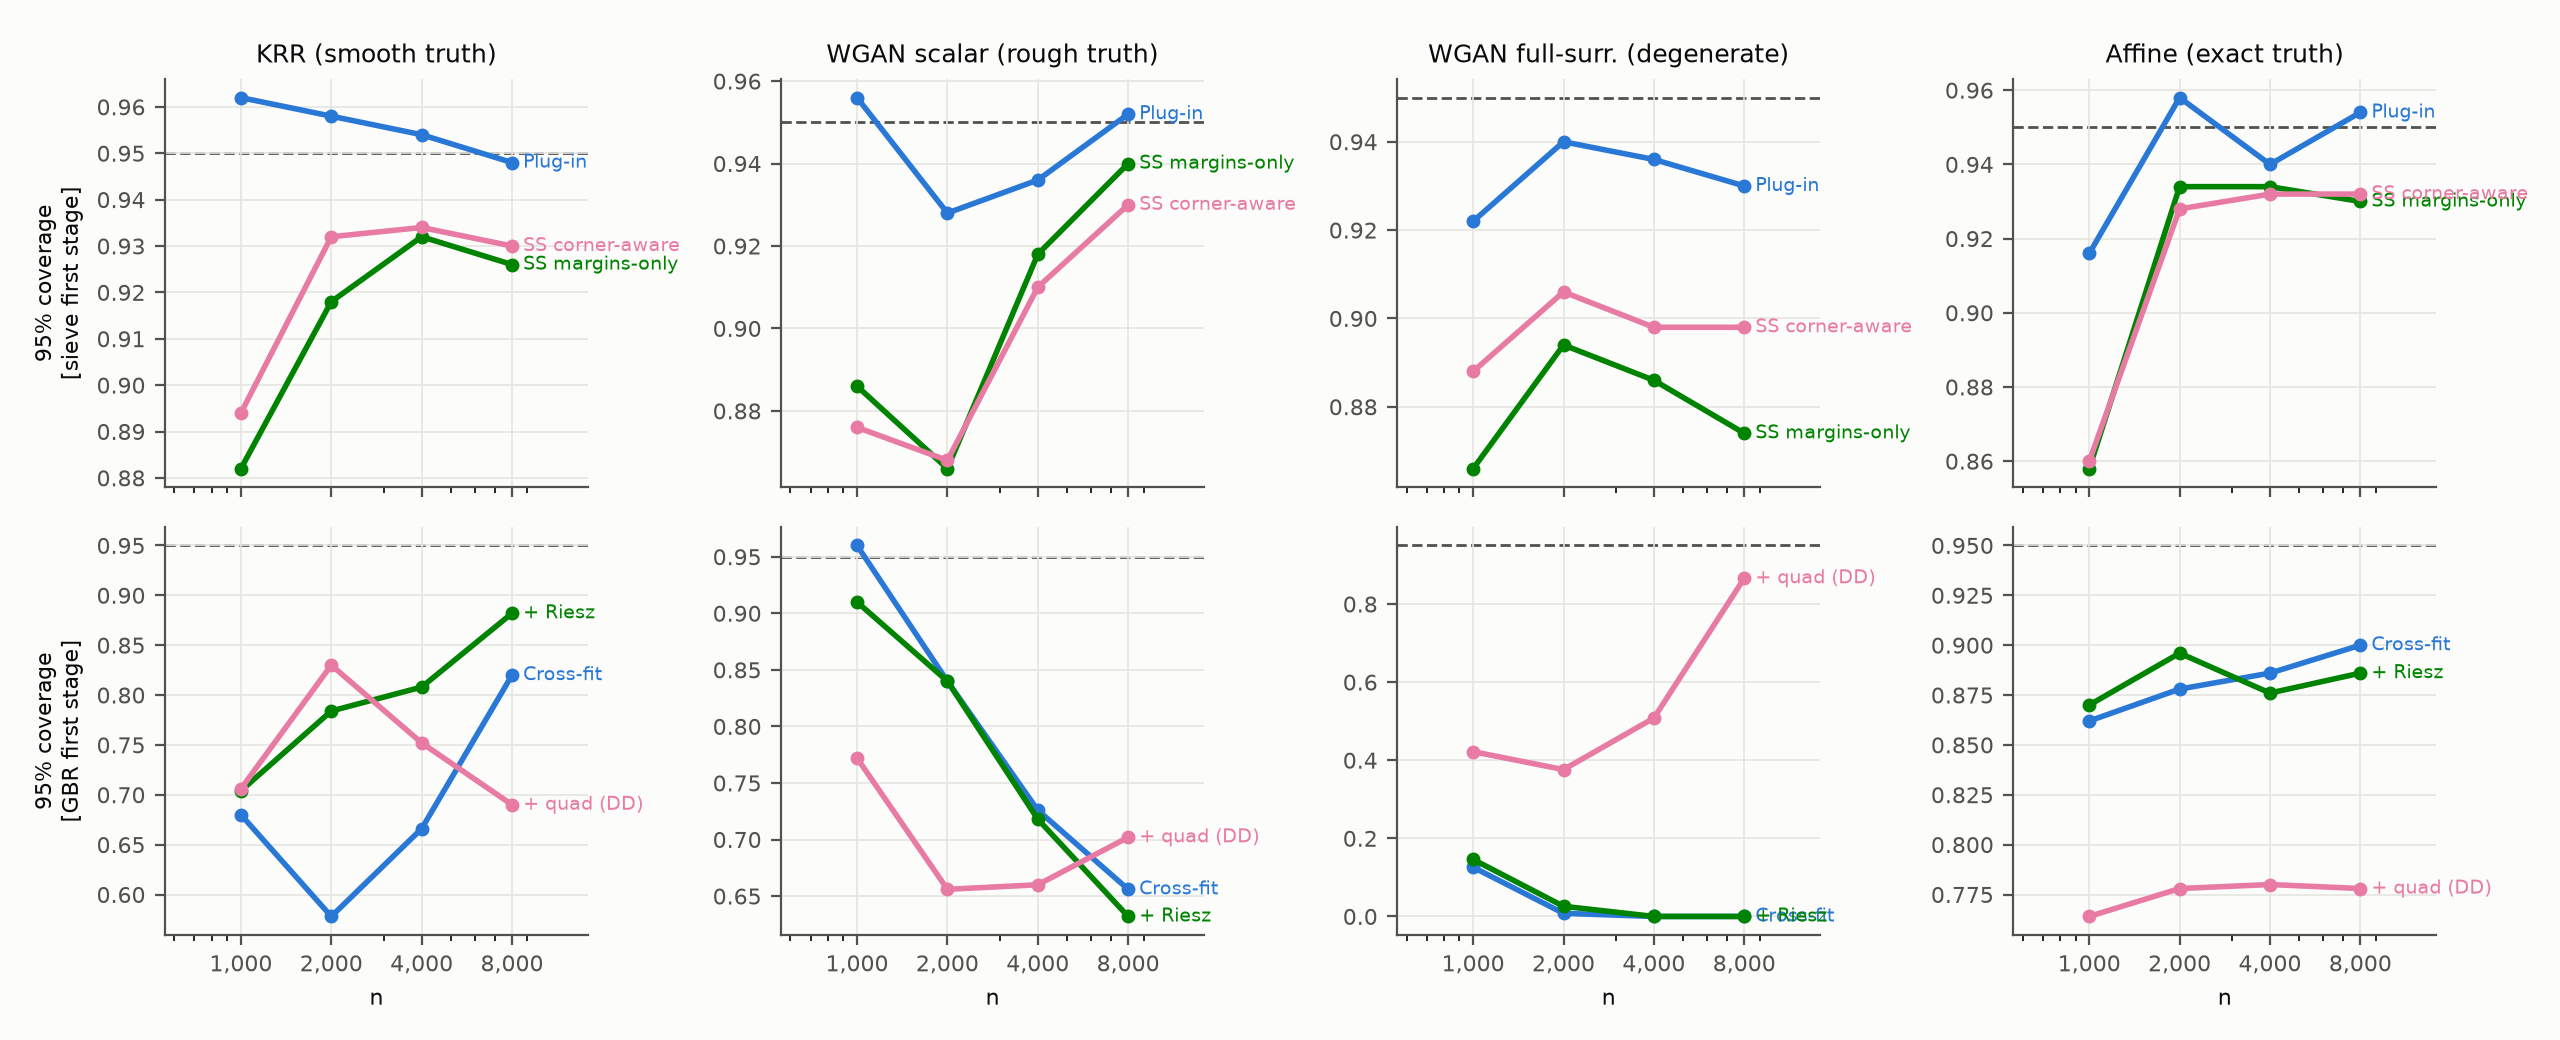
\includegraphics[width=\textwidth]{fig_debias_coverage.png}
\caption{Empirical 95\% coverage by sample size, DGP (columns), and
first-stage family (rows). Dashed line: nominal $0.95$.}
\label{fig:coverage}
\end{figure}

\begin{figure}[!htbp]
\centering
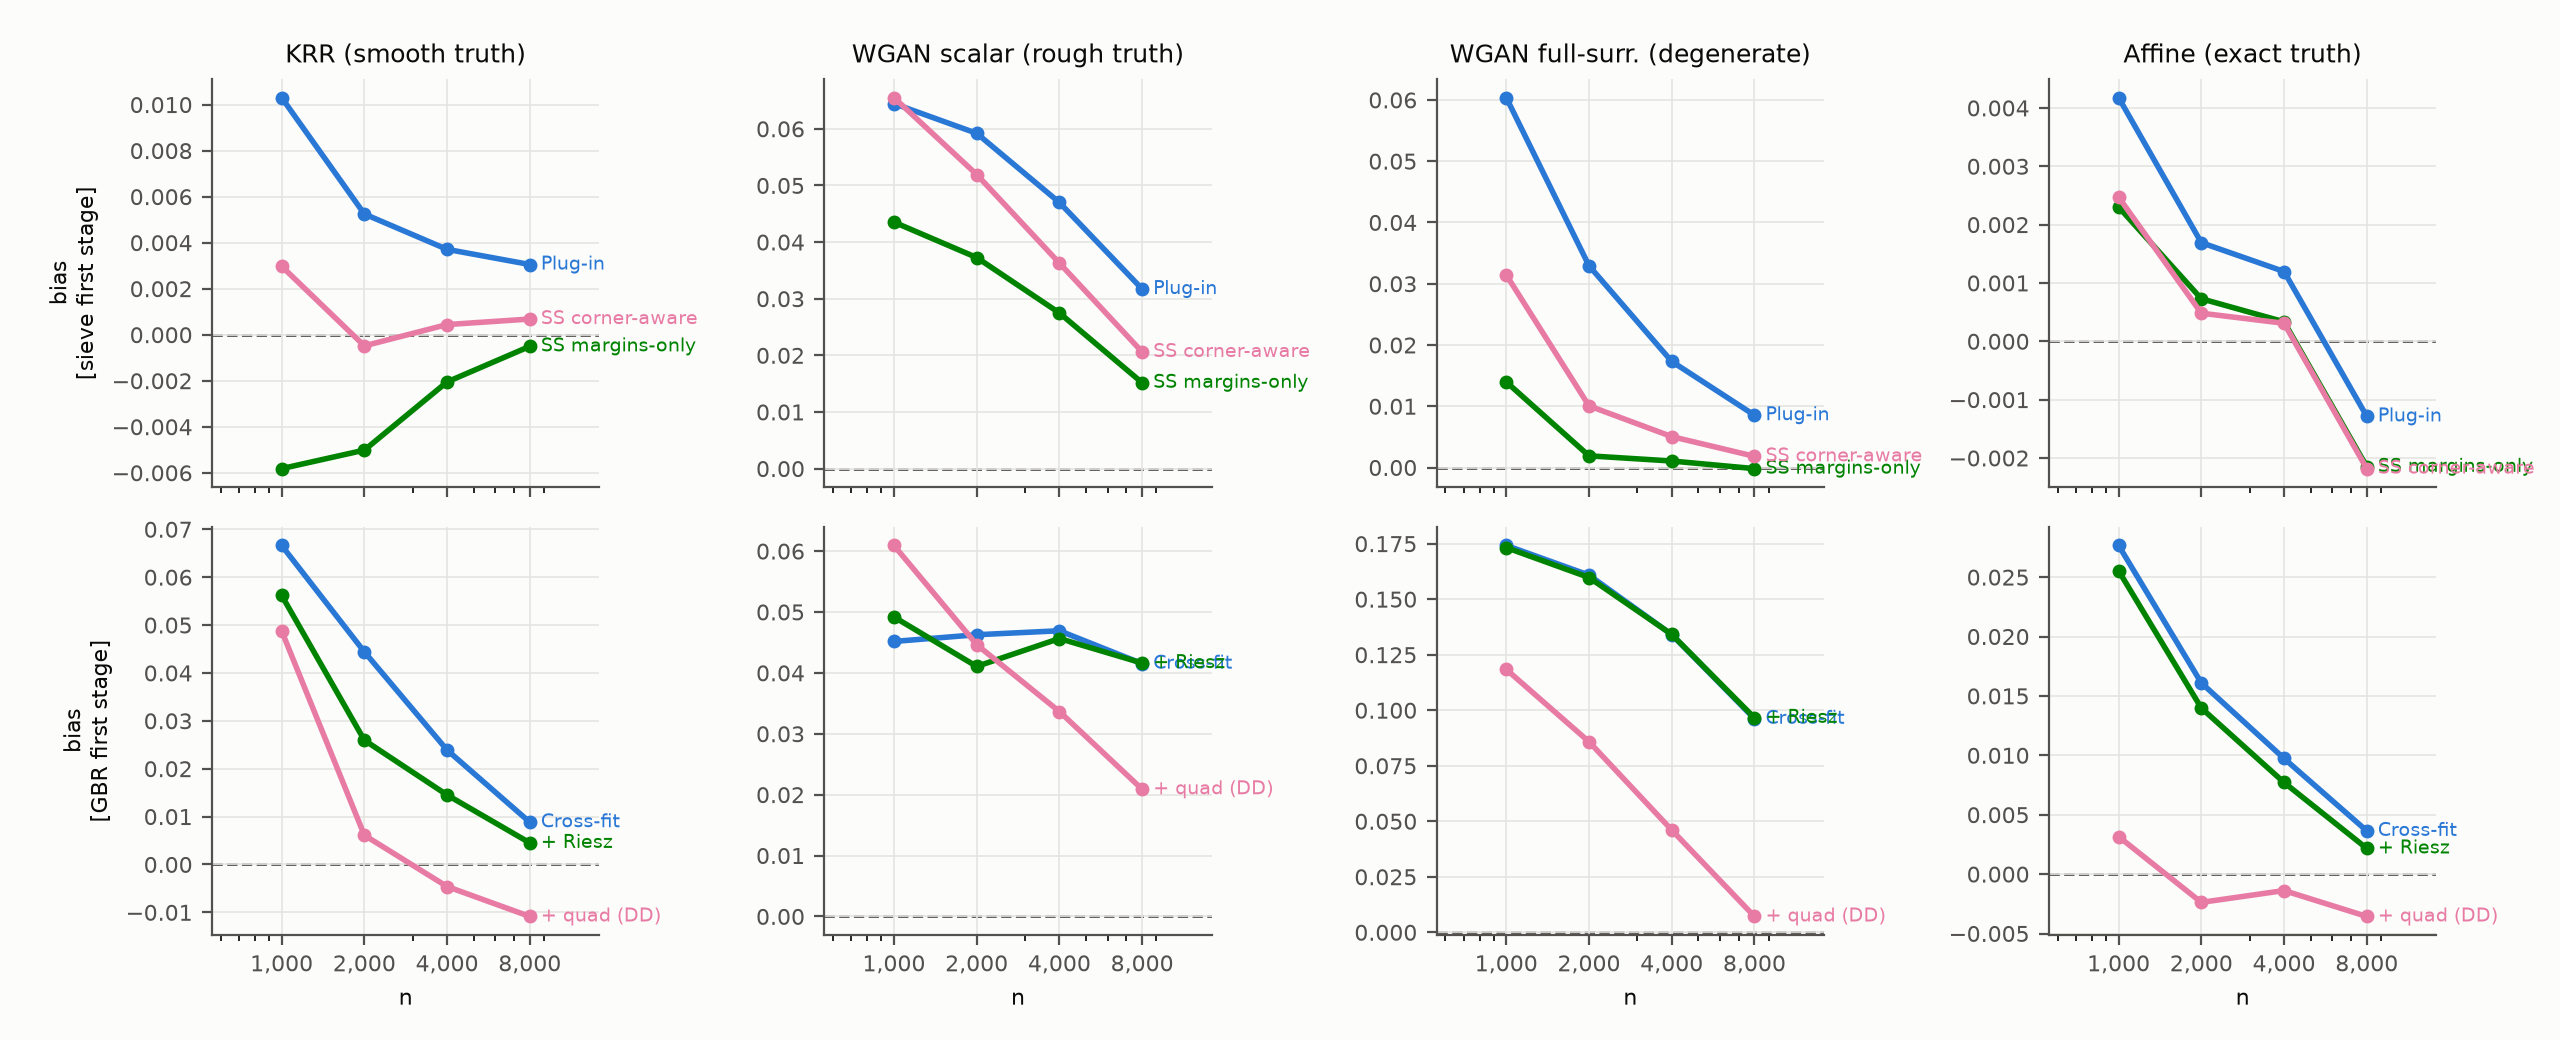
\includegraphics[width=\textwidth]{fig_debias_bias.png}
\caption{Monte Carlo bias by sample size, DGP, and estimator. Dashed
line: zero.}
\label{fig:bias}
\end{figure}

\begin{table}[!htbp]
\centering
\caption{Decomposition of the machine-learning undercoverage on the KRR
design ($n=4000$, $300$ replications). ``Plug-in bias'' is the uncorrected
cross-fit bias; ``bias'', ``SD'', ``SE/SD'', and ``coverage'' refer to the
Riesz-corrected estimator, studentized by \eqref{eq:two-band-var}. The
tensor-sieve plug-in is the reference. Varying folds, learner, and
representer basis one at a time isolates each mechanism of
Remark~\ref{rem:outofspan}. MC standard error of a coverage figure is about
$0.013$ at $300$ replications.}
\label{tab:dml-diag}
\begin{tabular}{lccccc}
\toprule
Configuration & Bias & Plug-in bias & SD & SE/SD & Coverage \\
\midrule
tensor-sieve plug-in & +0.0034 & +0.0034 & 0.0178 & 1.03 & 0.943\\
gbr K=2 riesz=sieve & +0.0216 & +0.0317 & 0.0186 & 0.96 & 0.760\\
gbr K=5 riesz=sieve & +0.0106 & +0.0160 & 0.0191 & 0.94 & 0.903\\
gbr K=10 riesz=sieve & +0.0079 & +0.0127 & 0.0196 & 0.92 & 0.913\\
rf K=5 riesz=sieve & +0.0119 & +0.0453 & 0.0195 & 1.01 & 0.907\\
krr K=5 riesz=sieve & +0.0038 & +0.0039 & 0.0184 & 0.90 & 0.917\\
gbr K=5 riesz=rf & +0.0078 & +0.0160 & 0.0203 & 0.96 & 0.937\\
krr K=5 riesz=rf & +0.0047 & +0.0039 & 0.0181 & 0.98 & 0.937\\
gbr(high-cap) K=5 riesz=sieve & +0.0439 & +0.0461 & 0.0131 & 1.00 & 0.077\\
gbr K=5 no correction & +0.0160 & +0.0160 & 0.0189 & 0.94 & 0.857\\
\bottomrule
\end{tabular}
\end{table}

\begin{figure}[!htbp]
\centering
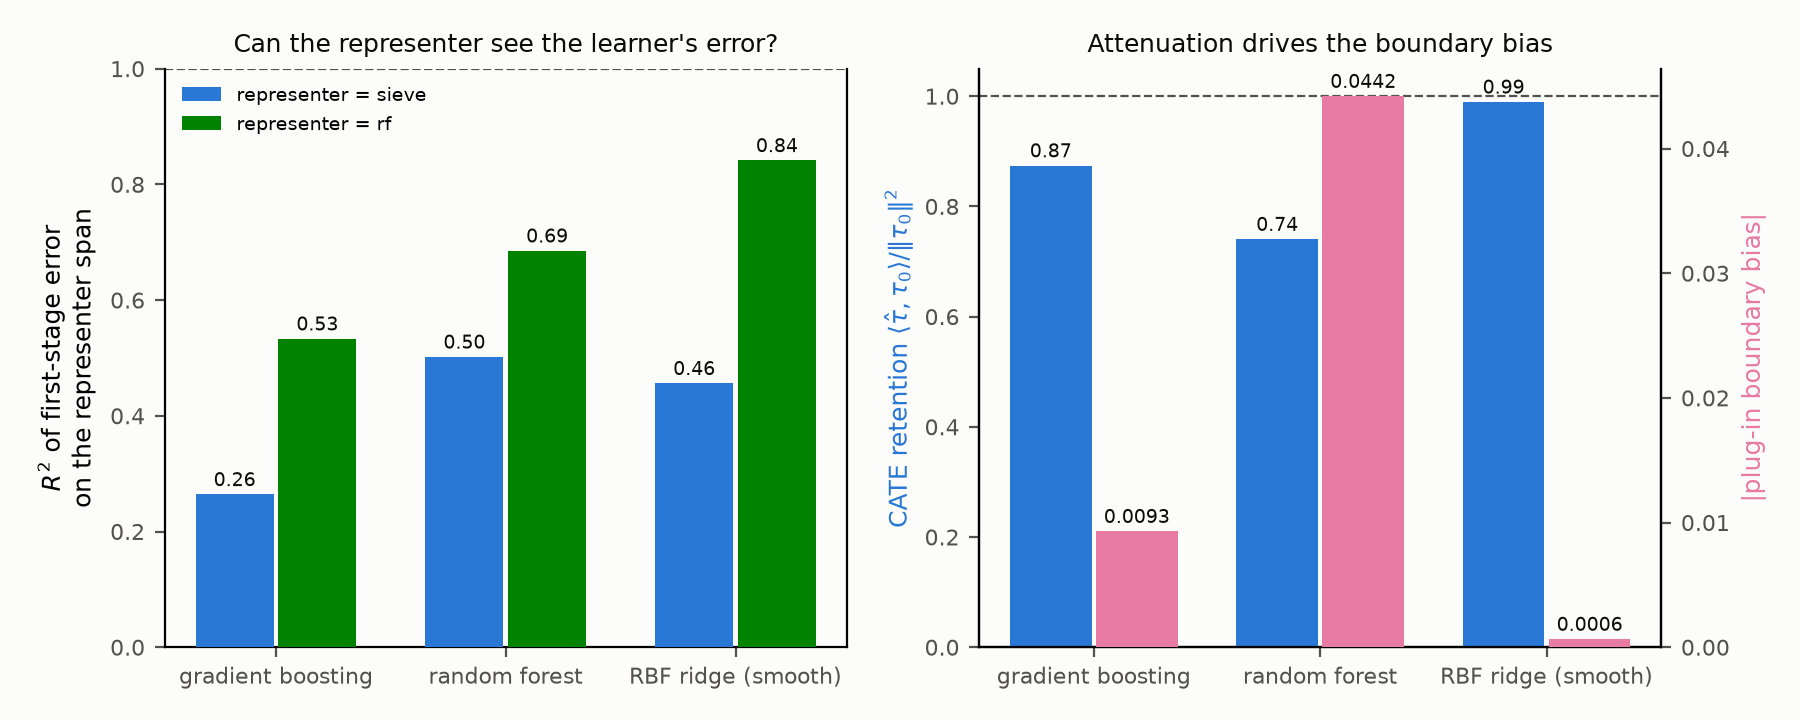
\includegraphics[width=\textwidth]{fig_dml_diagnosis.png}
\caption{Why boosting-based DML undercovers. \emph{Left}: the fraction
($R^{2}$) of the first-stage error that the sieve-Riesz representer can
span in global $L^{2}$, measured against the oracle arm means; a boosted-tree
error is largely invisible to a smooth representer, a random-feature ridge's
error is not. \emph{Right}: tree learners attenuate the CATE
(no-intercept projection coefficient of fitted on true, $\hat\tau'\tau/
\tau'\tau<1$), which displaces the decision boundary and biases the
plug-in; the smooth learner barely attenuates and is nearly unbiased. Both
panels average five simulated datasets and are indicative rather than
precise.}
\label{fig:dml-diag}
\end{figure}

\subsection{Corner anatomy}
\label{sec:anatomy}

Because the KRR oracle's contrast surfaces are known in closed form, the
corner set and its geometry are computable: the zero curves of $\tau_{S}$ and
$\tau_{Y}$ cross at ten points, with gradient norms
$\norm{\nabla\tau_{S}}\in[10.3,135.8]$, $\norm{\nabla\tau_{Y}}\in[13.9,56.4]$,
$\abs{\cos\omega}\leq0.90$ (transversality holds:
$\abs{\sin\omega}\geq0.45$), and within-unit residual correlation
$\rho_{SY}=0.524$. Table~\ref{tab:anatomy} traces the corner mechanism of
Section~\ref{sec:orders} across $300$ replications per sample size (sieve
first stage, fixed $K$).

\begin{table}[!htbp]
\centering
\caption{Corner anatomy on the KRR-calibrated oracle (300 reps, fixed
sieve dimension). ``Total'' is the implied plug-in corner bias
$\sum_{x^{*}}\E[\Delta_{g}\Delta_{h}]\,w/
(\Ng\Nh\abs{\sin\omega})$ in $\theta$ units;
``SS estimate'' is the mean corner cross correction
$\widehat{\text{corner}}$ of \eqref{eq:polarization}, which by split-sample
independence targets the \emph{stochastic} ($K/n$) part of the
diagonal; ``remainder'' is their difference, the bias-product
($K^{-2s/d}$) part. Sign convention: the anatomy script measures
$\E[\Delta\hat\tau_{S}\,\Delta\hat\tau_{Y}]$ (positive here, as
$\rho_{SY}>0$); the table reports the corner term in $\theta$ units, where
the harm-share convention $h_{0}=-\tau_{Y}$ flips its sign.
$\overline{\text{corr}}$ averages
$\mathrm{Corr}(\Delta_{g}(x^{*}),\Delta_{h}(x^{*}))$ over the ten corners.
The column implements the corner \emph{cross} term
$\mathcal B_{\Corner}^{\times}$ of Proposition~\ref{prop:margins} --- the
first term of the bracket in \eqref{eq:corner-coef} --- which by
\eqref{eq:polar-limit} is exactly the quantity that margins-only debiasing
leaves behind and that $\widehat{\mathrm{corner}}$ targets, so the comparison
across columns is like-for-like. It is \emph{not} the corner's full
contribution to the plug-in bias, which also contains the two
$\cos\omega$-weighted diagonals of \eqref{eq:corner-coef} (non-negligible
here, since $\abs{\cos\omega}$ reaches $0.90$) but which margins-only
debiasing already removes. The column also uses an unnormalized covariate
density (Section~\ref{sec:limits}, item~(L2)).}
\label{tab:anatomy}
\begin{tabular}{lccccc}
\toprule
$n$ & Total corner bias & SS estimate & Remainder &
$\overline{\text{corr}}(\Delta_{g},\Delta_{h})$ & $\rho_{SY}$\\
\midrule
2000 & $-0.0080$ & $-0.0044$ & $-0.0036$ & $0.50$ & $0.524$\\
4000 & $-0.0048$ & $-0.0022$ & $-0.0025$ & $0.46$ & $0.524$\\
8000 & $-0.0038$ & $-0.0012$ & $-0.0026$ & $0.45$ & $0.524$\\
\bottomrule
\end{tabular}
\end{table}

Three predictions of Section~\ref{sec:orders} are consistent with the table.
\emph{(i)} The pointwise correlation of the two surface errors at the corner
tracks the within-unit residual correlation ($0.45$--$0.50$ against
$\rho_{SY}=0.524$), which is the mechanism behind the $V_{gh}$ term in
\eqref{eq:corner-coef}. \emph{(ii)} The stochastic part of the corner
diagonal halves as $n$ doubles at fixed $K$
($-0.0044\to-0.0022\to-0.0012$) --- the $K/n$ scaling --- and is tracked by
the SS corner correction, which by construction cancels bias parts across the
two independent halves. \emph{(iii)} The remainder is roughly constant in $n$
at fixed $K$ ($-0.0036$ at $n=2000$, then $\approx-0.0025$), as befits the
$K^{-2s/d}$ bias product, which is controlled by undersmoothing $K$ rather
than by debiasing --- and which, per Proposition~\ref{prop:margins}, the SS
statistic is not supposed to capture. The measured corner bias
($0.4$--$0.8$ percentage points of a $\theta_{0}=0.161$ target)
is material relative to the plug-in standard error, and its sign matches the
Monte Carlo finding that the corner-aware and margins-only SS estimates
differ by $+0.004$ to $+0.005$ at $n=2000$. This validates the cross-corner
component of \eqref{eq:corner-coef} --- the component that
Proposition~\ref{prop:margins} says is at stake in the margins-only
comparison. The two $\cos\omega$ components of \eqref{eq:corner-coef} are not
tested here, because both debiasing variants remove them; testing them would
require comparing the \emph{plug-in} against a corner-corrected plug-in.

\subsection{Results}\label{sec:results}

Table~\ref{tab:mc-main} and Figures~\ref{fig:coverage}--\ref{fig:bias}
report all cells; Section~\ref{sec:limits} states which conclusions they can
and cannot support.

\emph{(1) Smooth truth (KRR): the plug-in is already good; corner-aware SS
removes what bias there is.} The plug-in covers at $0.948$--$0.962$ at all
$n$ with a small decaying bias ($+0.010\to+0.003$) and a well-calibrated
standard error (SE/SD $0.94$--$1.11$, tightening toward one with $n$). SS
debiasing removes the bias essentially completely ($+0.003\to+0.0007$; a
$3.5$-fold bias reduction at $n=1000$ and a tenfold reduction at $n=2000$)
at negligible variance cost by $n\geq4000$. The
\emph{margins-only} correction overshoots to negative bias
($-0.006$ to $-0.0005$) at every $n$: it removes the (positive) margin
diagonals --- and, per \eqref{eq:polar-limit}, the two $\cos\omega$ corner
diagonals as well --- but not the (negative) corner \emph{cross} term. The gap
between the corner-aware and margins-only estimates equals the estimated
corner correction ($\hat\Th_{SS}=\hat\Th_{SS}^{\text{mar}}
-\widehat{\text{corner}}$) and matches the anatomy of
Table~\ref{tab:anatomy} to the fourth decimal ($+0.0045$ at $n=2000$
against minus the anatomy's SS corner estimate of $-0.0044$).
The raw corner cross form $q_{\text{full}}-q_{g}-q_{h}$ (eight times the
corner correction) halves as $n$ doubles
($-0.070\to-0.036\to-0.020\to-0.0095$) at fixed $K$, the $K/n$ scaling of
\eqref{eq:corner-coef}. Coverage of the SS intervals is $0.894$--$0.934$
on this design: an improvement in centering bought at a $2$--$5$ point
coverage cost relative to the plug-in, which we do not describe as honest
coverage.

\emph{(2) Rough truth (scalar WGAN, $s\approx1$): debiasing accelerates the
bias decay.} This design violates the smoothness hypothesis of every theorem
above ($s\approx1<(d+1)/2=1.5$), so it is a robustness probe. The plug-in
bias is large and decays at only $\approx n^{-0.34}$ ($+0.064\to+0.032$),
and its near-nominal coverage rests on a conservative SE (SE/SD
$1.1$--$1.3$). SS debiasing accelerates the empirical decay to
$\approx n^{-0.55}$ ($+0.066\to+0.021$) with SE/SD $0.83$--$0.98$ and
coverage $0.87\to0.93$. Because $K$ is fixed across $n$ here, these
exponents describe the finite-sample behavior of the estimators at $K=25$;
they are not estimates of the asymptotic rate, which would require
$K_{n}$ to grow (Section~\ref{sec:limits}, item~(L4)). On this rough truth
the margins-only variant is slightly better centered than the corner-aware
one --- with $s\approx1$ the corner correction is itself noisily estimated
--- a useful caution: corner-awareness is a bias-\emph{decomposition}
necessity, but its sampled version adds noise when the surfaces are rough.

\emph{(3) Machine-learning first stages: the projected Riesz correction
works where the learner is adequate; the quadratic correction is not a free
lunch.} On the smooth truth the GBR bias falls monotonically along the
ladder cross-fit $\to$ $+$Riesz $\to$ $+$quadratic at every $n$ (at
$n=4000$: $+0.024\to+0.015\to-0.005$), consistent with the two corrections
targeting distinct error terms. But the composition has two finite-sample
costs: the SS-on-GBR quadratic correction inflates the dispersion (by a
factor of two at $n=1000$, $1.4$ thereafter), and the first-order SE does
not account for it (SE/SD $\approx0.6$), so DD
intervals undercover ($0.69$--$0.83$); and at $n=8000$ on KRR the
quadratic correction overshoots ($-0.011$). This is what
Remark~\ref{rem:tree-jack} predicts: \eqref{eq:jackknife} is a fourth-order
finite difference of a function that, for tree first stages, is a step
function, so Theorem~\ref{thm:dd} simply does not apply to this cell. On the
rough truth GBR is bias-limited ($+0.045$ nearly flat in $n$; coverage falls
to $0.64$): no first-order correction can rescue a nuisance that misses the
kinks. The degenerate arm is the extreme case: GBR manufactures a spurious
harm share of $+0.17$ (coverage $0$), and there the quadratic correction
\emph{does} rescue it ($+0.007$, coverage $0.87$ at $n=8000$).

\emph{(4) The two-band SE is well calibrated for the sieve family.} The
variance estimator \eqref{eq:two-band-var} includes the empirical-measure
term $\hat\varsigma^{2}/n=\hat\theta(1-\hat\theta)/n$ --- the sampling error
of the average given the surfaces, the analogue of the
$\mathrm{Var}([h_{0}]_{+})$ term the single-threshold unknown-density welfare
theorem adds --- which is $6$--$12\%$ of the SE at these sample sizes and, if
omitted, produces a spurious SE/SD of $0.87$--$0.95$. With it included,
SE/SD is $0.90$--$1.11$ for plug-in and SS on the KRR and affine designs, and
the studentized intervals reach $0.93$--$0.95$ by $n=8000$; on the
degenerate arm ($\theta_{0}=0$, empty margins) the sieve family degrades
gracefully.

\emph{(5) Machine-learning first stages: why the sieve-DML interval
undercovers, and when it does not.} The cross-fitted GBR estimators cover
only $0.58$--$0.88$ on the smooth design, in sharp contrast to the sieve
plug-in on the \emph{same samples} --- so the shortfall is a property of the
first stage, not the DGP or the variance formula. The diagnosis is
Remark~\ref{rem:outofspan}. Measured against the oracle arm means, the
$R^{2}$ of the boosted first-stage error on the tensor B-spline representer
span is $0.21$--$0.34$ across the four arm regressions (mean $0.26$); the
projected correction removes $31\%$ of the plug-in's boundary bias. The
direct variance test reported in Remark~\ref{rem:outofspan} shows that the
remaining $69\%$ is \emph{bias}, not an independent added variance: the
leading explanation is that the correction cannot see the part of the
learner's error that lives on the margins, so it leaves the boundary
displaced. Three levers move coverage:
\emph{(i) folds} --- $K=2\to5\to10$ lifts GBR coverage $0.76\to0.90\to0.91$
by shrinking the own-observation bias trained on $(K-1)/K$ of the sample;
\emph{(ii) representer basis} --- matching a $400$-feature random-feature
representer to the boosted learner raises the projected $R^{2}$ from $0.26$
to $0.53$ and coverage from $0.90$ to $0.94$; \emph{(iii) learner
smoothness} --- a random-feature (RBF) ridge, whose error the representer
\emph{can} span ($R^{2}=0.84$), attenuates the CATE by only about $1\%$
(against boosting's $13\%$) and has a plug-in bias of $+0.0006$ (against
$+0.016$), so there is almost nothing left to correct and, with a matched
representer, it too reaches $0.94$. Higher-capacity boosting is
counterproductive --- it sharpens the axis-aligned staircase, driving
coverage toward zero. The pattern reproduces the parent draft's own
single-threshold Table~7. The residual $0.01$--$0.02$ shortfall of even the
best machine-learning cell below the sieve plug-in's coverage is within
two Monte Carlo standard errors and should not be over-interpreted.

\subsection{What the current Monte Carlo does and does not
establish}\label{sec:limits}

The tables above are reproduced from v1 without change. Auditing the code
against the theory turned up six implementation gaps. None of them affects
Theorem~\ref{thm:D2} or the order accounting of Section~\ref{sec:orders},
which are analytic; all of them bear on how much weight the simulation
evidence can carry, and all are scheduled for repair before the next
revision. We list them explicitly rather than leave them implicit.

\begin{description}[leftmargin=2.2em,style=nextline]
\item[(L1) The KRR ``oracle truth'' is displaced by uncentered residual
resampling.] The sampler draws outcome noise by resampling the fitted
per-arm KRR residual pools, which are not centered (ridge shrinkage leaves
arm-specific residual means). The generated conditional means therefore
differ from the nominal KRR surfaces by a constant per arm, shifting the
generated CATEs by $\Delta\tau_{S}=+0.126$ and $\Delta\tau_{Y}=+0.182$
(the latter includes the short$\to$long coupling). The reported truth
$\theta_{0}$ moves from $0.16115$ to $0.15998$ --- immaterial for the bias
columns --- but the ten corner locations, gradients, angles, and first-stage
errors used in Table~\ref{tab:anatomy} are all computed against the
\emph{wrong} surfaces. Fix: center each arm's residual pool before
resampling, or define the oracle truth to include the shifts.
\item[(L2) The corner density is unnormalized.] Covariates are drawn from
the KDE conditional on $X\in[-3,3]^{2}$ by rejection sampling, but the
density accessor returns the untruncated KDE. The KDE mass of the box is
$0.807$, so the corner integrals in Table~\ref{tab:anatomy} should be scaled
by $1/0.807\approx1.24$ before any comparison with
\eqref{eq:corner-coef}. Together with the omission of the $\cos\omega$ terms
noted in the table caption, the ``Total'' column is an incomplete
implementation of the theory it is meant to check.
\item[(L3) The KRR design violates Assumption~\ref{ass:geometry}(d).] The
KDE density is positive at the truncation boundary, and a direct scan of the
four box edges finds twelve sign crossings of the two contrast surfaces
($\tau_{S}$: three on $x_{1}=-3$, two on $x_{1}=+3$, three on $x_{2}=-3$;
$\tau_{Y}$: two on $x_{1}=-3$, two on $x_{2}=+3$). The margins therefore
terminate at the support edge, and by Remark~\ref{rem:edge} the correct
second derivative for this DGP carries additional support-edge
$\Haus^{d-2}$ terms that \eqref{eq:D2} omits. Fix: taper $w$ near
$\partial\mathcal X$, or shrink the box so that all margins close inside it.
\item[(L4) The main Monte Carlo holds $K$ fixed.] Every sample size uses two
knot segments per coordinate, i.e.\ $K=25$ basis functions per arm at every
$n$. The design therefore does not implement
$K_{n}\asymp n^{d/(2s+1)}$, and the estimated log-rate slopes reported in
Section~\ref{sec:results}(2) are not estimates of the asymptotic rate. What
the design \emph{does} deliver cleanly is the $K/n$ scaling of the corner
diagonal at fixed $K$ (Table~\ref{tab:anatomy}), which is the prediction
Section~\ref{sec:orders} is actually testing.
\item[(L5) The variance bandwidth does not satisfy
Proposition~\ref{prop:var}.] The implementation sets
$\varepsilon=\delta\cdot\widehat{\mathrm{sd}}(\hat\tau)$ with $\delta$ fixed
and then widens $\varepsilon$ by factors of $1.5$ until at least five
observations enter the band. Since $\widehat{\mathrm{sd}}(\hat\tau)$
converges to a positive constant, $\varepsilon_{n}\not\to0$, contradicting
Proposition~\ref{prop:var} and Assumption~\ref{ass:dml}(b). On the
degenerate arm the widening manufactures a nonempty derivative band where
the population margin is empty. Fix: $\varepsilon_{n}=\delta_{n}\cdot
\widehat{\mathrm{sd}}(\hat\tau)$ with $\delta_{n}\to0$ at a rate satisfying
$n\varepsilon_{n}/K_{n}\to\infty$.
\item[(L6) The coded Riesz correction is not fold-specific.] Both the
cross-fitted DML estimator and the DD estimator build a single full-sample
Gram matrix and band representer from pooled out-of-fold predictions, whereas
\eqref{eq:dml} and Theorem~\ref{thm:dml} require an off-fold representer for
each fold. In the implementation, observation $i$'s outcome can influence the
global band through the model trained on $i$'s own fold, which breaks the
conditional mean-zero step used in Remark~\ref{rem:outofspan}. Fix: build
$\hat v^{*}_{-\kappa}$ inside the fold loop.
\end{description}

Taken together: Theorem~\ref{thm:D2} is verified analytically
(Appendix~\ref{app:numeric}); the $K/n$ order of the corner diagonal and the
sign and magnitude of the corner correction are supported by
Tables~\ref{tab:anatomy} and~\ref{tab:mc-main} at $d=2$ and fixed $K$,
subject to (L1)--(L3); the asymptotic rate claims of
Theorems~\ref{thm:plugin}, \ref{thm:ss}, \ref{thm:dml} and~\ref{thm:dd} are
\emph{not} tested by the present design, because $K$ does not grow with $n$;
and the mechanism behind the machine-learning undercoverage is identified as
residual boundary bias rather than unmodelled variance, by the direct
variance test in Remark~\ref{rem:outofspan}.

\emph{Practical guidance.} For sieve first stages, use the corner-aware SS
estimator \eqref{eq:jackknife} with the two-band SE: it is tuning-free and
removes the second-order stochastic diagonal including the corner, at a
$2$--$5$ point coverage cost relative to the plug-in in our designs. For a
machine-learning first stage --- needed when $d$ is too large for a tensor
sieve --- prefer a \emph{smooth} learner and \emph{match the representer
basis to the learner's own feature map}, so the projected correction is
near-exact; avoid tree ensembles, whose piecewise-constant error is largest
precisely on the margins the representer must span, and use at least five
folds for the nuisance cross-fit. (This is guidance about the number of
\emph{nuisance} folds and does not conflict with the two-half construction of
$\hat\Th_{SS}$ and $\hat\Th_{DD}$: there, the two halves furnish the
independent replicates that the polarization identity \eqref{eq:ss-identity}
requires, and $K=2$ is not a cross-fitting choice but part of the definition
of the quadratic correction. The two can be combined --- $K$-fold nuisance
cross-fitting inside each half --- at the cost of one more fit.) When a tree
first stage is unavoidable, pair it with a full-refit bootstrap rather than
the analytic SE. The comparison of the corner-aware and margins-only
corrections is a useful specification diagnostic in its own right: their gap
estimates the corner cross term, whose magnitude flags whether the
two-threshold structure is quantitatively binding.

\appendix

\section{Derivation of the Second Derivative (Theorem~\ref{thm:D2})}
\label{app:D2}

Write $T_{g}(t):=\int_{\{g_{t}=0\}\cap\{h_{t}\geq0\}}
\varpi_{t}\dd\Haus^{d-1}$ with weight
$\varpi_{t}:=u\,w/\norm{\nabla g_{t}}$ (we reserve $\omega(x)$ for the
transversality angle throughout), the first term of \eqref{eq:D1}
along $\gamma_{t}$; the second term is symmetric. Let
${\bf X}(\cdot,t)$ be the normal diffeomorphism carrying
$\mathcal M:=\{g_{0}=0\}$ to $\{g_{t}=0\}$ with velocity
$\dot{\bf X}=-(u/\Ng)\,n_{g}$, and pull the integral back
to $\mathcal M$:
\[
T_{g}(t)=\int_{\mathcal M}
\1\{h_{t}({\bf X}(x,t))\geq0\}\;
\varpi_{t}({\bf X}(x,t))\,J_{\bf X}(x,t)\dd\Haus^{d-1}(x).
\]
Differentiating at $t=0$ yields four contributions.
\emph{(1) Integrand:} $\partial_{t}\varpi_{t}
=-u\,w\,(n_{g}\!\cdot\!\nabla u)/\Ng^{2}$.
\emph{(2) Transport of $\varpi$ and area:} by the surface-transport formula
\citep[Ch.~9]{dz2001},
$\partial_{t}\{\varpi({\bf X})J_{\bf X}\}
=-\big[(u/\Ng)\,n_{g}\!\cdot\!\nabla\varpi
+\varpi\,(u/\Ng)H_{g}\big]$, the moving-level-set terms of
\citet[Lem.~PathD--Level]{cg2026} with weight $\varpi$.
\emph{(3) Direct motion of the cut:} the indicator
$\1\{h_{t}\geq0\}$ evaluated on the (fixed, $t=0$) manifold defines the
region $\{h_{0}+tv\geq0\}\cap\mathcal M$; by the within-manifold Leibniz
rule its derivative is an integral over the relative boundary
$\Corner$ with normal velocity $v/\norm{\nabla_{\!\mathcal M}h_{0}}$, where
$\norm{\nabla_{\!\mathcal M}h_{0}}=\norm{P_{T}\nabla h_{0}}
=\Nh\abs{\sin\omega}$, giving
$+\int_{\Corner}\varpi_{0}\,v/(\Nh\abs{\sin\omega})
\dd\Haus^{d-2}$ --- the cross term.
\emph{(4) Induced motion of the cut:} the composition
$h_{0}({\bf X}(x,t))=h_{0}(x)-t\,(u/\Ng)\,
n_{g}\!\cdot\!\nabla h_{0}+o(t)
=h_{0}(x)-t\,u\,\Nh\cos\omega/\Ng+o(t)$
perturbs the cut function by an effective
$v_{\text{eff}}=-u\Nh\cos\omega/\Ng$;
the same within-manifold Leibniz rule then contributes
$-\int_{\Corner}\varpi_{0}\,u\cos\omega/
(\Ng\abs{\sin\omega})\dd\Haus^{d-2}$ --- the diagonal
corner term of \eqref{eq:Qg}. Collecting (1)--(4), and adding the symmetric
derivative of the $\Mh$-term (which contributes the mirror-image margin
form, the second copy of the cross term, and the $v^{2}$ diagonal corner
term), gives \eqref{eq:D2}--\eqref{eq:Qg}. Transversality bounds every
corner integrand; twice-differentiability of $g_{0},h_{0}$ and
Assumption~\ref{ass:model}(d) bound the curvature and gradient terms.
$\hfill\square$

\section{Orders of the Remainder Terms}\label{app:proofs}

The margin components of all remainder bounds are adaptations of the
single-threshold arguments --- \citet[Thms.~5, 8 and the SS/LOO
constructions]{cg2026} for the quadratic terms, and the extended
single-threshold draft (sieve-DML theorem and its Assumption~5) for the
cross-fitted first-order correction --- applied margin by margin with the
truncation indicators carried as bounded weights. This appendix records the
two order calculations that are specific to the two-threshold geometry and
that v1 got wrong.

\subsection*{B.1 Why the margin diagonal is $K_{n}^{1+1/d}/n$}

Substituting the stochastic part \eqref{eq:decomp} into $Q_{g}$ and
separating $i=j$ from $i\neq j$,
\[
Q_{g}[u_{g},u_{g}]
=\underbrace{\frac1{n^{2}}\sum_{i}\epsilon_{S,i}^{2}\,Q_{g}[s_{i},s_{i}]}
_{T_{\mathrm{diag}}}
+\underbrace{\frac1{n^{2}}\sum_{i\neq j}\epsilon_{S,i}\epsilon_{S,j}\,
Q_{g}[s_{i},s_{j}]}_{T_{\mathrm{off}}} .
\]
The leading integrand of $Q_{g}$ carries one gradient, so
$\E\,Q_{g}[s_{i},s_{i}]$ involves
$\E[s_{i}(x)\,n_{g}\!\cdot\!\nabla s_{i}(x)]
=b(x)'G^{-1}\nabla b(x)\cdot n_{g}\asymp K_{n}^{1+1/d}$ by
\eqref{eq:sieve-scaling}, whence
$\E\,T_{\mathrm{diag}}\asymp n^{-2}\cdot n\cdot K_{n}^{1+1/d}
=K_{n}^{1+1/d}/n$. This is the order stated by \citet{cg2026} for
the single-threshold value functional, and it is the order that
Table~\ref{tab:orders} records. The curvature part of $Q_{g}$, which carries
no gradient, contributes only $K_{n}/n$.

The corner forms in \eqref{eq:D2}--\eqref{eq:Qg} carry \emph{no} gradient of
$u$ or $v$. Their diagonals therefore involve
$\E[s_{i}(x)^{2}]=b(x)'G^{-1}b(x)=\mathcal V(x)\asymp K_{n}$ and are
$K_{n}/n$: bounded by $K_{n}^{-1/d}$ times the margin bound. v1's assertion
that the corner diagonal is ``of the same order $K_{n}/n$ as the margin
diagonals'' conflated a bound with an exact order.

Two asymmetries between the two statements should be recorded.
\emph{(i)} The corner order is exact: $\mathcal V>0$ and enters
undifferentiated, so integrating it over $\Corner$ against a weight of
constant sign cannot cancel. \emph{(ii)} The margin order is a bound only.
$\E[s_{i}\,\partial_{n}s_{i}]=\tfrac12\partial_{n}\mathcal V$ under
homoskedasticity, and $\mathcal V$ oscillates at the mesh scale with
amplitude $\asymp K_{n}$, so while $\norm{\nabla\mathcal V}_{\infty}\asymp
K_{n}^{1+1/d}$ pointwise, the surface integral in \eqref{eq:gradV} can
cancel. Expanding $\mathcal V=\bar{\mathcal V}+\tilde{\mathcal V}$ with
$\tilde{\mathcal V}$ mesh-periodic and mean zero, and writing
$\tilde{\mathcal V}(x)=\sum_{j\neq0}c_{j}e^{2\pi ij\varkappa^{-1}x}$, the
integral of $\partial_{n}\mathcal V$ along a margin of slope $\alpha$ (in
$d=2$) picks up a non-decaying contribution only from pairs $(j,l)$ with
$j+l\alpha\approx0$, i.e.\ only if $\alpha$ is rational with small
denominator; for cubic splines $\abs{c_{j}}=O(j^{-4})$, so even moderate
denominators are heavily suppressed. Appendix~\ref{app:numeric}, item~5,
confirms this: $\alpha\in\{0,1\}$ give $\asymp K_{n}^{1+1/d}$,
$\alpha\in\{1/2,8/5\}$ and irrational $\alpha$ give $\asymp K_{n}$.
Consequently the margin bound is attained for mesh-resonant margins ---
in particular for $d=1$, where $\Mg$ is a point and no averaging occurs, so
the single-threshold rate of \citet{cg2026} is unaffected --- but not
necessarily otherwise.

\subsection*{B.2 Off-diagonal (cross-half) orders}

$T_{\mathrm{off}}$ is a degenerate second-order $U$-statistic. Writing
$a_{i}:=G^{-1}b(X_{i})$, every quadratic form in \eqref{eq:D2} evaluates to
$a_{i}'Ma_{j}$ for a symmetric matrix $M$ built from the relevant boundary
integral, so
$\mathrm{Var}(T_{\mathrm{off}})\asymp n^{-2}\,\mathrm{tr}\{(MG^{-1})^{2}\}$.
For tensor B-splines with mesh $\varkappa=K_{n}^{-1/d}$, a normalized basis
function has height $\asymp\varkappa^{-d/2}$ on a cell of volume
$\varkappa^{d}$, so for a $p$-dimensional integration set $\mathcal S$ and
$\ell$ gradient factors,
\[
\#\{k: \mathrm{supp}(b_{k})\cap\mathcal S\neq\emptyset\}\asymp\varkappa^{-p},
\qquad
M_{kk}\asymp\varkappa^{-d}\varkappa^{p}\varkappa^{-\ell}
=\varkappa^{p-d-\ell},
\]
and therefore $\mathrm{tr}(M^{2})\asymp\varkappa^{-p}\varkappa^{2(p-d-\ell)}
=\varkappa^{p-2d-2\ell}=K_{n}^{(2d+2\ell-p)/d}$. Substituting:
\begin{center}
\begin{tabular}{lccl}
\toprule
Term & $(p,\ell)$ & $\mathrm{tr}(M^{2})$ & $T_{\mathrm{off}}$ \\
\midrule
margin, gradient part & $(d-1,1)$ & $K_{n}^{(d+3)/d}$
  & $n^{-1}K_{n}^{(d+3)/(2d)}$\\
corner & $(d-2,0)$ & $K_{n}^{(d+2)/d}$
  & $n^{-1}K_{n}^{(d+2)/(2d)}$\\
margin, curvature part & $(d-1,0)$ & $K_{n}^{(d+1)/d}$
  & $n^{-1}K_{n}^{(d+1)/(2d)}$\\
\bottomrule
\end{tabular}
\end{center}
The first line reproduces the $n^{-1}\sqrt{K_{n}^{(d+3)/d}}$ bound of
\citet{cg2026}, which is a useful check on the calculus. Two
consequences. First, all three are $O(r_{n}^{*})$ at
$K_{n}\asymp n^{d/(2s+1)}$ under $s\geq(d+1)/2$ (the corner needs only
$s\geq d/2$), so the off-diagonals never bind before the terms in
Table~\ref{tab:orders}'s third block do. Second, and correcting v1: it is
\emph{not} true in general that a lower-dimensional integration set gives a
smaller cross-half term. Reducing $p$ by one \emph{raises}
$\mathrm{tr}(M^{2})$ by $K_{n}^{1/d}$, because there is less averaging, not
more. Comparing like with like, the codimension-two corner has a
\emph{larger} generic off-diagonal than a hypersurface with the same
integrand. The corner off-diagonal ends up smaller than the leading margin
off-diagonal only because the margin form carries a gradient factor
($\ell=1$) that costs $K_{n}^{2/d}$ in $\mathrm{tr}(M^{2})$, which more than
offsets the corner's $K_{n}^{1/d}$ dimension gain; it remains
\emph{larger} than the margin's curvature part.

\subsection*{B.3 Status of the proofs}

The joint CLT for the two-band linear term follows from the Cram\'er--Wold
device and the Lindeberg--Lyapunov condition of Assumption~\ref{ass:dml}(g)
applied to the summed per-unit influence
$v^{*}_{S}(X_{i},W_{i})\epsilon_{S,i}+v^{*}_{Y}(X_{i},W_{i})\epsilon_{Y,i}$;
the within-unit correlation $\rho_{SY}$ is absorbed into $\sigma_{n}^{2}$ by
construction \eqref{eq:two-band-var}. Beyond the order calculations of B.1
and B.2, complete proofs of Theorems~\ref{thm:ss}, \ref{thm:dml}
and~\ref{thm:dd} are not yet written; the statements above are formulated so
that the cited single-threshold lemmas apply to the margin parts verbatim,
and the corner parts require only the transversality bound and the dimension
count $\dim\Corner=d-2$. The two places where this is not merely mechanical
are (i) the uniform control of the estimated geometry along the jackknife
path (Assumption~\ref{ass:path}), which is an assumption rather than a
result, and (ii) the moving-boundary remainder
Assumption~\ref{ass:dml}(f), whose primitive sufficient conditions for
generic machine-learning first stages we do not currently have.

\section{Numerical Verification of Theorem~\ref{thm:D2}}\label{app:numeric}

Theorem~\ref{thm:D2} was checked against exact area computations in $d=2$ on
four designs, chosen so that between them every term of
\eqref{eq:D2}--\eqref{eq:Qg} is activated in isolation. In each case
$\Th(t)=\int\1\{g_{0}+tu\geq0\}\1\{h_{0}+tv\geq0\}w$ has a closed form;
$\Th''(0)$ is obtained by a Richardson-extrapolated central second difference
and compared with the right-hand side of \eqref{eq:D2}.

\begin{enumerate}[leftmargin=2em]
\item \emph{Radially weighted disk.} $g_{0}=1-\norm{x}^{2}$, no second
threshold, $w=\rho(\norm{x})$, $u\equiv a$. Only the transport and curvature
terms of $Q_{g}$ are active, and \eqref{eq:Qg} reduces to
$\pi a^{2}\rho'(1)/2$. Relative error $6\times10^{-10}$.
\item \emph{Disk with a non-constant direction.} $g_{0}=1-\norm{x}^{2}$,
$w\equiv1$, $u(x)=\norm{x}^{2}$, so $\{g_{t}\geq0\}$ is the disk of radius
$(1-t)^{-1/2}$ and $\Th(t)=\pi/(1-t)$. This activates the
$u\,(n_{g}\!\cdot\!\nabla u)$ term. Formula and truth both give
$D\Th=\pi$, $D^{2}\Th=2\pi$ to ten digits.
\item \emph{Disk cut by an oblique chord.} $g_{0}=1-\norm{x}^{2}$,
$h_{0}=x_{1}-\kappa$, $w\equiv1$, $u\equiv a$, $v\equiv c$. Both margin
forms vanish, isolating the two corner diagonals and the corner cross term at
$\cos\omega=-\kappa$. Checked at $\kappa\in\{0.6,0.2,-0.5\}$ (both signs of
$\cos\omega$) and $(a,c)\in\{(1,1),(1.7,-0.9),(0.4,2.1)\}$; maximum relative
error $2\times10^{-10}$.
\item \emph{Lens of two disks.} $g_{0}=1-\norm{x-p}^{2}$,
$h_{0}=1-\norm{x-q}^{2}$ with $\norm{p-q}=D$, $w\equiv1$, $u\equiv a$,
$v\equiv c$; both surfaces curved and obliquely intersecting, with
$\cos\omega=1-D^{2}/2$. The prediction
$\{ac-\tfrac12(a^{2}+c^{2})\cos\omega\}/\abs{\sin\omega}$ matches the exact
lens area's second derivative at $D\in\{0.8,1.2,1.7\}$ and the same three
$(a,c)$ pairs; maximum relative error $2\times10^{-9}$.
\end{enumerate}

Designs 3 and 4 are the substantive ones. Varying $(a,c)$ over three
non-proportional pairs identifies the quadratic form in $(a,c)$ separately,
so they confirm all three coefficients
\[
\underbrace{\frac{2}{\Ng\Nh\abs{\sin\omega}}}_{\text{cross}},
\qquad
\underbrace{\frac{-\cos\omega}{\Ng^{2}\abs{\sin\omega}}}_{Q_{g}\text{ diag.}},
\qquad
\underbrace{\frac{-\cos\omega}{\Nh^{2}\abs{\sin\omega}}}_{Q_{h}\text{ diag.}},
\]
and their relative signs, at both signs of $\cos\omega$.

The sharpest single check is design 4 with a \emph{one-sided} perturbation,
$v\equiv0$: there the cross term is identically zero, so anything nonzero
must come from the $Q_{g}$ corner diagonal. At $D=0.8,1.2,1.7$
($\cos\omega=+0.680,+0.280,-0.445$) and $a=1$ the exact lens curvatures are
$-0.463713017$, $-0.145833333$, $+0.248456065$, against formula values
$-0.463713017$, $-0.145833333$, $+0.248456064$ --- including the sign
reversal as $\cos\omega$ crosses zero. This is the term that v1's order
discussion omitted and that \eqref{eq:corner-coef} restores: the corner
contributes to the plug-in bias even when the two contrast errors are
uncorrelated, provided the margins do not meet orthogonally.

\medskip
\noindent\textbf{5. Polarization and mesh resonance.} Two further checks
support statements made in the body.

\emph{(a) The polarization identity \eqref{eq:polar-limit}.} On all thirteen
$(D\ \text{or}\ \kappa,\,a,\,c)$ configurations of designs 3 and 4, the
numerically differenced $q_{\text{full}}-q_{g}-q_{h}$ agrees with
$2C[a,c]$ to full double precision, while the sum of the two $\cos\omega$
diagonals --- which is nonzero and often larger in magnitude --- is absorbed
entirely into $q_{g}$ and $q_{h}$. For instance at $D=1.2$, $a=c=1$:
$q_{\text{full}}=0.750000$, $q_{g}=q_{h}=-0.145833$, so
$q_{\text{full}}-q_{g}-q_{h}=1.041667=ac/\abs{\sin\omega}=2C$, against a
corner-diagonal sum of $-0.291667$. This is what licenses
Proposition~\ref{prop:margins}: margins-only debiasing removes the
$\cos\omega$ diagonals and leaves the cross term.

\emph{(b) Mesh resonance in \eqref{eq:gradV}.} With periodic uniform cubic
tensor B-splines on the torus in $d=2$ ($K_{n}=m^{2}$, mesh
$\varkappa=1/m$), we computed $\mathcal V=\mathcal V_{1}\otimes\mathcal V_{1}$
in closed form --- the diagnostic $\int_{0}^{1}\mathcal V_{1}=m$ holds
exactly and $\norm{\mathcal V_{1}'}_{\infty}=1.226\,m^{2}$ to four digits for
$m=16,32,64$, confirming the pointwise scalings \eqref{eq:sieve-scaling}
--- and evaluated $\int_{\Mg}\psi\,\partial_{n}\mathcal V$ along straight
margins of slope $\alpha$ for $m=16,32,64,128$. Reporting
$\abs{I}/K_{n}$ (flat $\Rightarrow$ $I\asymp K_{n}$; growing linearly in
$m$ $\Rightarrow$ $I\asymp K_{n}^{1+1/d}$):
\begin{center}
\begin{tabular}{lcccc}
\toprule
$\alpha$ & $m=16$ & $32$ & $64$ & $128$\\
\midrule
$0$ (mesh-aligned) & 16.1 & 20.7 & 66.6 & 27.4 \\
$1$ (resonant) & 3.6 & 5.2 & 15.4 & 6.9 \\
$1/2$, $8/5$ (rational, $q\geq2$) & $\leq0.12$ & $\leq0.20$ & $\leq0.09$
  & $\leq0.59$\\
$1/\pi$, $\sqrt2$, $\sqrt5-1$ (irrational) & $\leq0.43$ & $\leq0.65$
  & $\leq0.40$ & $\leq0.48$\\
\bottomrule
\end{tabular}
\end{center}
The first two rows fluctuate in phase but grow with $m$ (so
$I\asymp K_{n}^{1+1/d}$); the last two are bounded (so $I\asymp K_{n}$). The
resulting hundredfold spread at $m=128$ is the evidence for
Remark~\ref{rem:cancel}.

\medskip
\noindent\textbf{6. The support-edge term of Remark~\ref{rem:edge}.} Take the
unit disk $g_{0}=1-\norm{x}^{2}$ with the \emph{fixed} support
$\mathcal X=\{x_{1}\geq\kappa\}$, $w\equiv1$, $u\equiv a$, and no second
threshold. The exact curvature of the circular-segment area matches
$-2a^{2}\cos\omega_{\partial}/(4\abs{\sin\omega_{\partial}})$ with
$\cos\omega_{\partial}=-\kappa$ at $\kappa\in\{0.6,0.2,0,-0.5\}$ and
$a\in\{1,1.7\}$ to ten digits, including the exact vanishing at $\kappa=0$
(orthogonal meeting). This confirms both the form of the edge term and that
it carries no cross component.

\medskip
The scripts for items 1--6 are \texttt{verify\_D2\_theorem.py},
\texttt{verify\_polarization.py} and \texttt{verify\_mesh\_resonance.py},
alongside this document.

\begin{thebibliography}{99}

\bibitem[Athey et al.(2024)Athey, Chetty, Imbens, and Kang]{acik2024}
Athey, S., R. Chetty, G.~W. Imbens, and H. Kang (2024): ``The Surrogate
Index: Combining Short-Term Proxies to Estimate Long-Term Treatment Effects
More Rapidly and Precisely,'' \emph{Working paper}.

\bibitem[Athey et al.(2021)Athey, Imbens, Metzger, and Munro]{aimm2021}
Athey, S., G.~W. Imbens, J. Metzger, and E. Munro (2021): ``Using Wasserstein
Generative Adversarial Networks for the Design of Monte Carlo Simulations,''
\emph{Journal of Econometrics}, forthcoming.

\bibitem[Banerjee et al.(2015)]{banerjee2015}
Banerjee, A., E. Duflo, N. Goldberg, D. Karlan, R. Osei, W. Pariente,
J. Shapiro, B. Thuysbaert, and C. Udry (2015): ``A Multifaceted Program
Causes Lasting Progress for the Very Poor: Evidence from Six Countries,''
\emph{Science}, 348(6236), 1260799.

\bibitem[Chen and Gao(2026)]{cg2026}
Chen, X., and W.~Y. Gao (2026): ``Thin Sets Are Not Equally Thin: Minimax
Learning of Submanifold Integrals,'' \emph{Working paper}; first version
arXiv:2507.12673v1.

\bibitem[Chen et al.(2025)Chen, Chen, and Gao]{ccg2025}
Chen, X., Z. Chen, and W.~Y. Gao (2025): ``Inference on Policy Value and
Welfare under Optimal Treatment Rules,'' \emph{Working paper}, and its
extended draft (quadratic debiasing; sieve DML).

\bibitem[Chen and Ritzwoller(2023)]{cr2023}
Chen, J., and D.~M. Ritzwoller (2023): ``Semiparametric Estimation of
Long-Term Treatment Effects,'' \emph{Journal of Econometrics}, 237(2),
105545.

\bibitem[Delfour and Zol\'esio(2001)]{dz2001}
Delfour, M.~C., and J.-P. Zol\'esio (2001): \emph{Shapes and Geometries:
Analysis, Differential Calculus, and Optimization}. SIAM, Philadelphia.

\bibitem[Evans and Gariepy(2015)]{eg2015}
Evans, L.~C., and R.~F. Gariepy (2015): \emph{Measure Theory and Fine
Properties of Functions}, revised ed. CRC Press, Boca Raton.

\bibitem[Viviano and Bradic(2024)]{viviano2024}
Viviano, D., and J. Bradic (2024): ``Fair Policy Targeting,'' \emph{Journal
of the American Statistical Association}, 119(545), 730--743.

\bibitem[Whitehouse et al.(2026)]{whitehouse2026}
Whitehouse, J., Q. Chen, M. Austern, and V. Syrgkanis (2026): ``Inference on
Optimal Policy Values and Other Irregular Functionals via Softmax
Smoothing,'' arXiv:2507.11780v2.

\end{thebibliography}

\end{document}
